\documentclass[Review,times,sageh]{sagej}

\usepackage{moreverb,url,natbib, multirow, tabularx}
\usepackage[hidelinks,bookmarksopen,bookmarksnumbered,citecolor=red,urlcolor=red]{hyperref}


% Pandoc citation processing

\usepackage{cleveref}
\providecommand{\tightlist}{\setlength{\itemsep}{0pt}\setlength{\parskip}{0pt}}



\begin{document}

\title{Multidimensional signals and analytic flexibility: Estimating degrees of freedom in human speech analyses}

\runninghead{Multidimensional signals and analytic flexibility}

\author{Stefano Coretta*\affilnum{1}, Joseph V. Casillas\affilnum{2}, Timo B. Roettger\affilnum{3}}

\affiliation{\affilnum{1}{Institute of Phonetics and Speech Processing, Ludwig-Maximilian University Munich, Germany.}\\\affilnum{2}{Department of Spanish and Portuguese, Rutgers University, New Brunswick, United States}\\\affilnum{3}{Department of Linguistics and Scandinavian Studies, University of Oslo, Oslo, Norway}}

\corrauth{Timo B. Roettger}

\email{\href{mailto:timo.b.roettger@iln.uio.no}{\nolinkurl{timo.b.roettger@iln.uio.no}}}

\begin{abstract}
Recent efforts to replicate published findings have uncovered surprisingly low success rates across disciplines. Moreover, several studies have highlighted the large degree of analytic flexibility in data analysis which can lead to substantially different conclusions based on the same data set. Thus, researchers have expressed their concerns that these researcher degrees of freedom might facilitate bias and can lead to claims that do not stand the test of time. Even greater flexibility is to be expected in fields in which the primary data lend themselves to a variety of possible operationalizations. The multidimensional, temporally extended nature of speech constitutes an ideal testing ground for assessing the variability in analytic approaches that derives not only from aspects of statistical modelling but also from decisions regarding the quantification of the measured behavior. In the present study, we will give the same speech production dataset to N teams of researchers and will ask them to answer the same research question. Using Bayesian meta-analytic tools, we will quantify this variability and relate it to predictors related to the analysts and their analyses.
\end{abstract}

\keywords{crowdsourcing science, data analysis, scientific transparency, speech, acoustic analysis}

\maketitle

\hypertarget{introduction}{%
\section{Introduction}\label{introduction}}

In order to effectively accumulate knowledge, science needs (i) to produce data that can be replicated using the original methods and (ii) to arrive at robust conclusions substantiated by such data.
In recent coordinated efforts to replicate published findings, scientific disciplines have uncovered surprisingly low success rates \citep[e.g.,][]{open2015estimating, camerer2018evaluating} leading to what is now referred to as the \emph{replication crisis}.
Beyond the difficulties of replicating scientific findings, a growing body of evidence suggests that researchers' conclusions often vary even when they have access to the same data.
The latter situation has been referred to as the \emph{inference crisis} \citep{rotello2015more, starns2019assessing} and is, among other things, rooted in the inherent flexibility of data analysis \citep[often referred to as researcher degrees of freedom:][]{simmons2011false, gelman2014statistical}.
Data analysis involves many different steps, such as inspecting, organizing, transforming, and modeling the data, to name a few.
Along the way, different methodological and analytic choices need to be made, all of which may influence the final interpretation of the data.

These researcher degrees of freedom are both a blessing and a curse.
They are a blessing because they afford us the opportunity to look at nature from different angles, which, in turn, allows us to make important discoveries and generate new hypotheses \citep[e.g.,][]{box1976science, tukey1977exploratory, de2014thought}.
They are a curse because idiosyncratic choices can lead to categorically different interpretations, which eventually find their way into the publication record where they are taken for granted \citep{simmons2011false}.
Recent projects have shown that the variability between different data analysts is vast and can lead independent researchers to draw different conclusions from the same data set \citep[e.g.,][]{silberzahn2018many, starns2019assessing, botvinik-nezer2020}.
These studies, however, might still underestimate the extent to which analysts vary because data analysis is not restricted to the statistical analysis of ready-made numeric data.
These data can in fact be the result of complex measurement processes that translate a phenomenon, such as human behavior, into numbers.
This is particularly true for fields that draw conclusions about human behavior and cognition from multidimensional data like audio or video data.
In fields working on human speech production, for example, researchers need to make numerous decisions about what to measure and how to measure it, in other words, how to operationalise the phenomenon under investigation.
This is not trivial, given the temporal extension of the acoustic signal and its complex structural composition.

In this article, we investigate the impact of analytic choices on research results when many analyst teams analyze the same speech production data set, a process that involves both decisions regarding the \emph{operationalization} of a complex signal and decisions regarding \emph{statistical analysis}.
Specifically, we discuss the degree of variability in research results obtained by N teams who had to choose the operationalisation and statistical procedures to answer the same research question, on the basis of the same set of raw data (here, speech recordings).
Our goals are twofold: (i) our study conceptually replicates previous many-analyses projects, by probing the effects of different statistical analyses and by assessing the generalizability of published findings to other disciplines (here, the speech sciences);
(ii) our study extends the scope of inquiry to include flexibility in the operationalisation of complex human behavior (here, human speech).
This is an important addition in that the increased number of ``forking paths'' in the ``garden of analytic choices'', deriving from the many decisions involved in quantification, might reveal a higher degree of variability across analysts than what previously observed, thus giving us a more realistic estimate of variability across analysts.

\hypertarget{researcher-degrees-of-freedom}{%
\subsection{Researcher degrees of freedom}\label{researcher-degrees-of-freedom}}

Data analysis comes with many decisions, for example how to measure a given phenomenon or behavior, which data to submit to statistical modeling and which to exclude in the final analysis, or what inferential decision-making procedure to apply.
This can be problematic because humans show cognitive biases that can lead to erroneous inferences.
Humans filter the world in irrational ways \citep[e.g.,][]{tversky1974judgment}, see coherent patterns in randomness \citep{brugger2001}, convince themselves of the validity of prior expectations \citep[``I knew it'',][]{nickerson1998confirmation}, and perceive events as being plausible in hindsight \citep[``I knew it all along'',][]{fischhoff1975hindsight}.
In conjunction with an academic incentive system that rewards certain discovery processes more than others \citep{sterling1959publication, koole2012rewarding}, we often find ourselves exploring many possible analytic pipelines, but only reporting a selected few.

This issue is particularly amplified in fields in which the raw data lend themselves to many possible ways of being measured \citep{roettger2019researcher}.
Combined with a wide variety of methodological and theoretical traditions as well as varying levels of quantitative training across subfields, the inherent flexibility of data analysis might lead to a vast plurality of analytic approaches that can lead to different scientific conclusions \citep{roettger2019emergent}.
Analytic flexibility has been widely discussed from a conceptual point of view \citep{simmons2011false, wagenmakers2012agenda, nosek2014method} and in regard to its application in individual scientific fields \citep[e.g.][]{wicherts2016, charles2019, roettger2019researcher}.
This notwithstanding, there are still many unknowns regarding the extent of analytic plurality in practice.

Consequently, it is likely that a good part of published papers present overconfident interpretations of data and statistical results based on idiosyncratic analytic strategies \citep[e.g.,][]{simmons2011false, gelman2014statistical}.
These interpretations, and the conclusions that derive from them, are thus associated with an unknown degree of uncertainty (dependent on the strength of evidence provided) and with an unknown degree of generalizability (dependent on the chosen analysis).
Moreover, the same data could lead to very different conclusions depending on the analytic path taken by the researcher.
However, instead of being critically evaluated, scientific results often remain unchallenged in the publication record.
Despite recent efforts to improve transparency and reproducibility \citep[e.g.][]{miguel2014promoting, klein2018practical} and the advent of freely available and accessible infrastructures, such as those provided by the Open Science Framework (osf.io), critical re-analyses of published analytic strategies are still uncommon because data sharing remains rare \citep{wicherts2006poor}.

\hypertarget{crowdsourcing-alternative-analyses}{%
\subsection{Crowdsourcing alternative analyses}\label{crowdsourcing-alternative-analyses}}

Recent collaborative attempts have started to shed light on how different analysts tackle the same data set and have revealed a large amount of variability.
In a seminal collaborative effort, \citet{silberzahn2018many} let twenty-nine independent analysis teams address the same research hypothesis.
Analytic approaches and consequently the results varied widely between teams.
Sixty-nine percent of the teams found support for the hypothesis, and 31\% did not.
Out of the 29 analytic strategies, there were 21 unique combinations of covariates.
Importantly, the observed variability was neither predicted by the team's preconceptions about the phenomenon under investigation nor by peer ratings of the quality of their analyses.

The authors results suggest that analytic plurality may be an inevitable byproduct of the scientific process and not necessarily driven by different levels of expertise or bias.

Several other recent studies corroborated this analytic flexibility across different disciplines.
\citet{dutilh2019} and \citet{starns2019assessing} investigated analysts' choices when inferring theoretical constructs based on the same data set using computational models.
Both studies revealed vastly different modeling strategies, even though scientific conclusions were similar across analysis teams (see also \citet{Parker2020} on analytic flexibility in ecology, and \citet{botvinik-nezer2020} on neuroimaging data).
\citet{bastiaansen2020} crowdsourced clinical recommendations based on analyses of an individual patient.
Their results suggests that analysts differed substantially regarding decisions related to both the statistical analysis of the data and the theoretical rationale behind interpreting the statistical results.

Extending on the many-analysts approach, \citet{landy2020crowdsourcing} asked 15 research teams to independently design studies to answer the same research questions.
Again, they found vast heterogeneity in researchers' conclusions which was not predicted by the researchers' expertise but seem to be more dependent on the research question itself.
This is in line with a recent re-analysis of \citet{silberzahn2018many} by \citet{auspurg2021has}.
The authors argue that the observed heterogeneity across analysts in \citet{silberzahn2018many} might have been driven by flexibility in statistically interpreting the research question.

While these studies attested a large degree of analytic flexibility with possibly impactful consequences, they focused on analytic decisions related to statistical inference or the architecture of computational models.
In these studies the data sets were fixed and neither data collection nor measurement could be changed.
Thus the estimates of variability found in the literature might reflect a lower bound only, ignoring large parts of the forking path related to measurement.

However, in many fields the primary raw data are complex signals that need to be operationalized relative to a theoretically motivated research question.
This is especially true in the social sciences, where the phenomenon under investigation corresponds to both observable and unobservable human behavior.

Decisions about how to measure a theoretical construct related to human behavior or its underlying cognitive processes might interact with downstream decisions about statistical modeling and vice versa.
For instance, \citet{flake2020} discuss the cascading impact that different practices can have on psychometric research.
The authors highlight, among others, the following degrees of freedom in the choice and development of measures: definition of the theoretical construct, justification of the selected measure, description of the measure and of how it maps onto the construct, response coding and related transformations, and post-hoc modifications to the chosen measure.
Taken together, these aspects alone dramatically increase the combinations of possible analytic choices, and hence flexibility in research outcomes.

In those disciplines concerned with communication, human behavior often corresponds to multidimensional visual and/or acoustic signals.
The complex nature of this data exponentiates the number of possible analytic approaches, thus further increasing analytic flexibility.
In order to estimate this increased flexibility, the present study looks at experimentally elicited speech production data.\\

\hypertarget{s:operspeech}{%
\subsection{Operationalizing speech}\label{s:operspeech}}

Research on speech lies at the intersection of the cognitive sciences, informing psychological models of language, categorization, and memory, guiding methods for diagnosis and therapy of speech disorders, and facilitating advancement in automatic speech recognition and speech synthesis.
One major challenge in the speech sciences is the mapping between communicative intentions (the unobserved behavior) and their physical manifestation (the observed behavior).

Speech is a complex signal that is characterized by structurally different acoustic landmarks distributed throughout different temporal domains.
Thus, choosing how to measure a communictive intention of interest is an important analytic step.
Take for example the following sentence in (1).

\vspace{1em}

\begin{enumerate}
\def\labelenumi{(\arabic{enumi})}
\tightlist
\item
  ``I can't bear another meeting on Zoom.''
  \vspace{1em}
\end{enumerate}

Depending on the speaker's intention, this sentence can be said in different ways.
For instance, if the speaker is exhausted by all their meetings, they might acoustically highlight the word \emph{another} or \emph{meeting} to contrast it with more pleasant activities.
If, on the other hand, the speaker is just tired of video conferences, as opposed to say face-to-face meetings, they might acoustically highlight the word \emph{Zoom}.

If we decide to compare the speech signal associated with these two intentions, how can we quantify the difference between them?
In other words, given their physical manifestation (speech), what do we measure and how do we measure it?
Because of the continuous and transient nature of speech, identifying speech parameters and temporal domains within which to measure those parameters becomes a non-trivial task.
Utterances stretch over several thousand milliseconds and contain different levels of linguistically relevant units such as phrases, words, syllables, and individual sounds.
The researcher is thus confronted with a considerable number of parameters and combinations thereof to choose from.

From a phonetic viewpoint, linguistically relevant units are inherently multidimensional and dynamic: they consist of clusters of parameters that are modulated over time.
The acoustic parameters of units are usually asynchronous, i.e.~they appear at different time points in the unfolding signal, and overlap with parameters of other units \citep[e.g.][]{jongman2000acoustic, lisker1986voicing, summerfield1981articulatory, winter2014spoken}.
A classical example is the distinction between voiced and voiceless stops in English (i.e.~/b/ and /p/ in \emph{bear} vs \emph{pear}).
This contrast is manifested by many acoustic features which can differ depending on several factors, such as position of the consonant in the word and surrounding sounds \citep{lisker1977rapid}.
Furthermore, correlates of the contrast can even be found away from the consonant, in temporally distant speech units.
For example, the initial /l/ of the English words \emph{led} and \emph{let} is affected by the voicing of the final consonant (/d, t/) \citep{hawkins2004influence}.

The multiplicity of phonetic measurements grows exponentially if we look at larger temporal domains as is the case for suprasegmental aspects of speech.
For example, studies investigating acoustic correlates of word stress (e.g.~the difference between \emph{ínsight} and \emph{incíte}) use a wide variety of measurements, including temporal characteristics (duration of certain segments or sub-segmental intervals), spectral characteristics (intensity, formants, and spectral tilt), and measurements related to fundamental frequency (f0) \citep[e.g.,][]{gordon2017acoustic}.
Moving on to the expression of higher-level communicative functions, like information structure and discourse pragmatics, relevant acoustic cues can be distributed throughout even larger domains, such as phrases and whole utterances \citep[e.g.,][]{ladd2008intonational}.
Differences in position, shape, and alignment of pitch modulations over multiple locations within a sentence are correlated with differences in discourse functions \citep[e.g.,][]{niebuhr2011}.
The latter can also be expressed by global vs local pitch modulations \citep{heuven2002}, as well as acoustic information within the temporal or spectral domain \citep[e.g.,][]{van2005speech}.
Extra-linguistic information, like the speaker's intentions, levels of emotional arousal or social identity, are also conveyed by broad-domain parameters, such as voice quality, rhythm, and pitch \citep{foulkes2006, ogden2004, white2009}.

In short, when testing hypotheses on speakers' intentions with speech production data, researchers are faced with many choices and possibilities.
The larger the functional domain (e.g.~segments vs words vs utterances), the higher the number of conceivable operationalizations.
For example, several decisions have to be made when comparing the two realizations of the sentence in (1), one of which is intended to signal emphasis on \emph{another} and one of which emphasizes \emph{Zoom} (see 2a and 2b).

\vspace{1em}

(2a) I can't bear \emph{ANOTHER} meeting on Zoom.

(2b) I can't bear another meeting on \emph{ZOOM}.

\vspace{1em}

Do we compare only the word \emph{another} in (2a) and (2b), or also the word \emph{Zoom}?
Do we measure utterance-wide acoustic profiles, whole words, or just stressed syllables?
Do we average across the chosen time domain or do we measure a specific point in time?
Do we measure fundamental frequency, intensity, or something else \citep{stevens2000}?



\begin{figure}
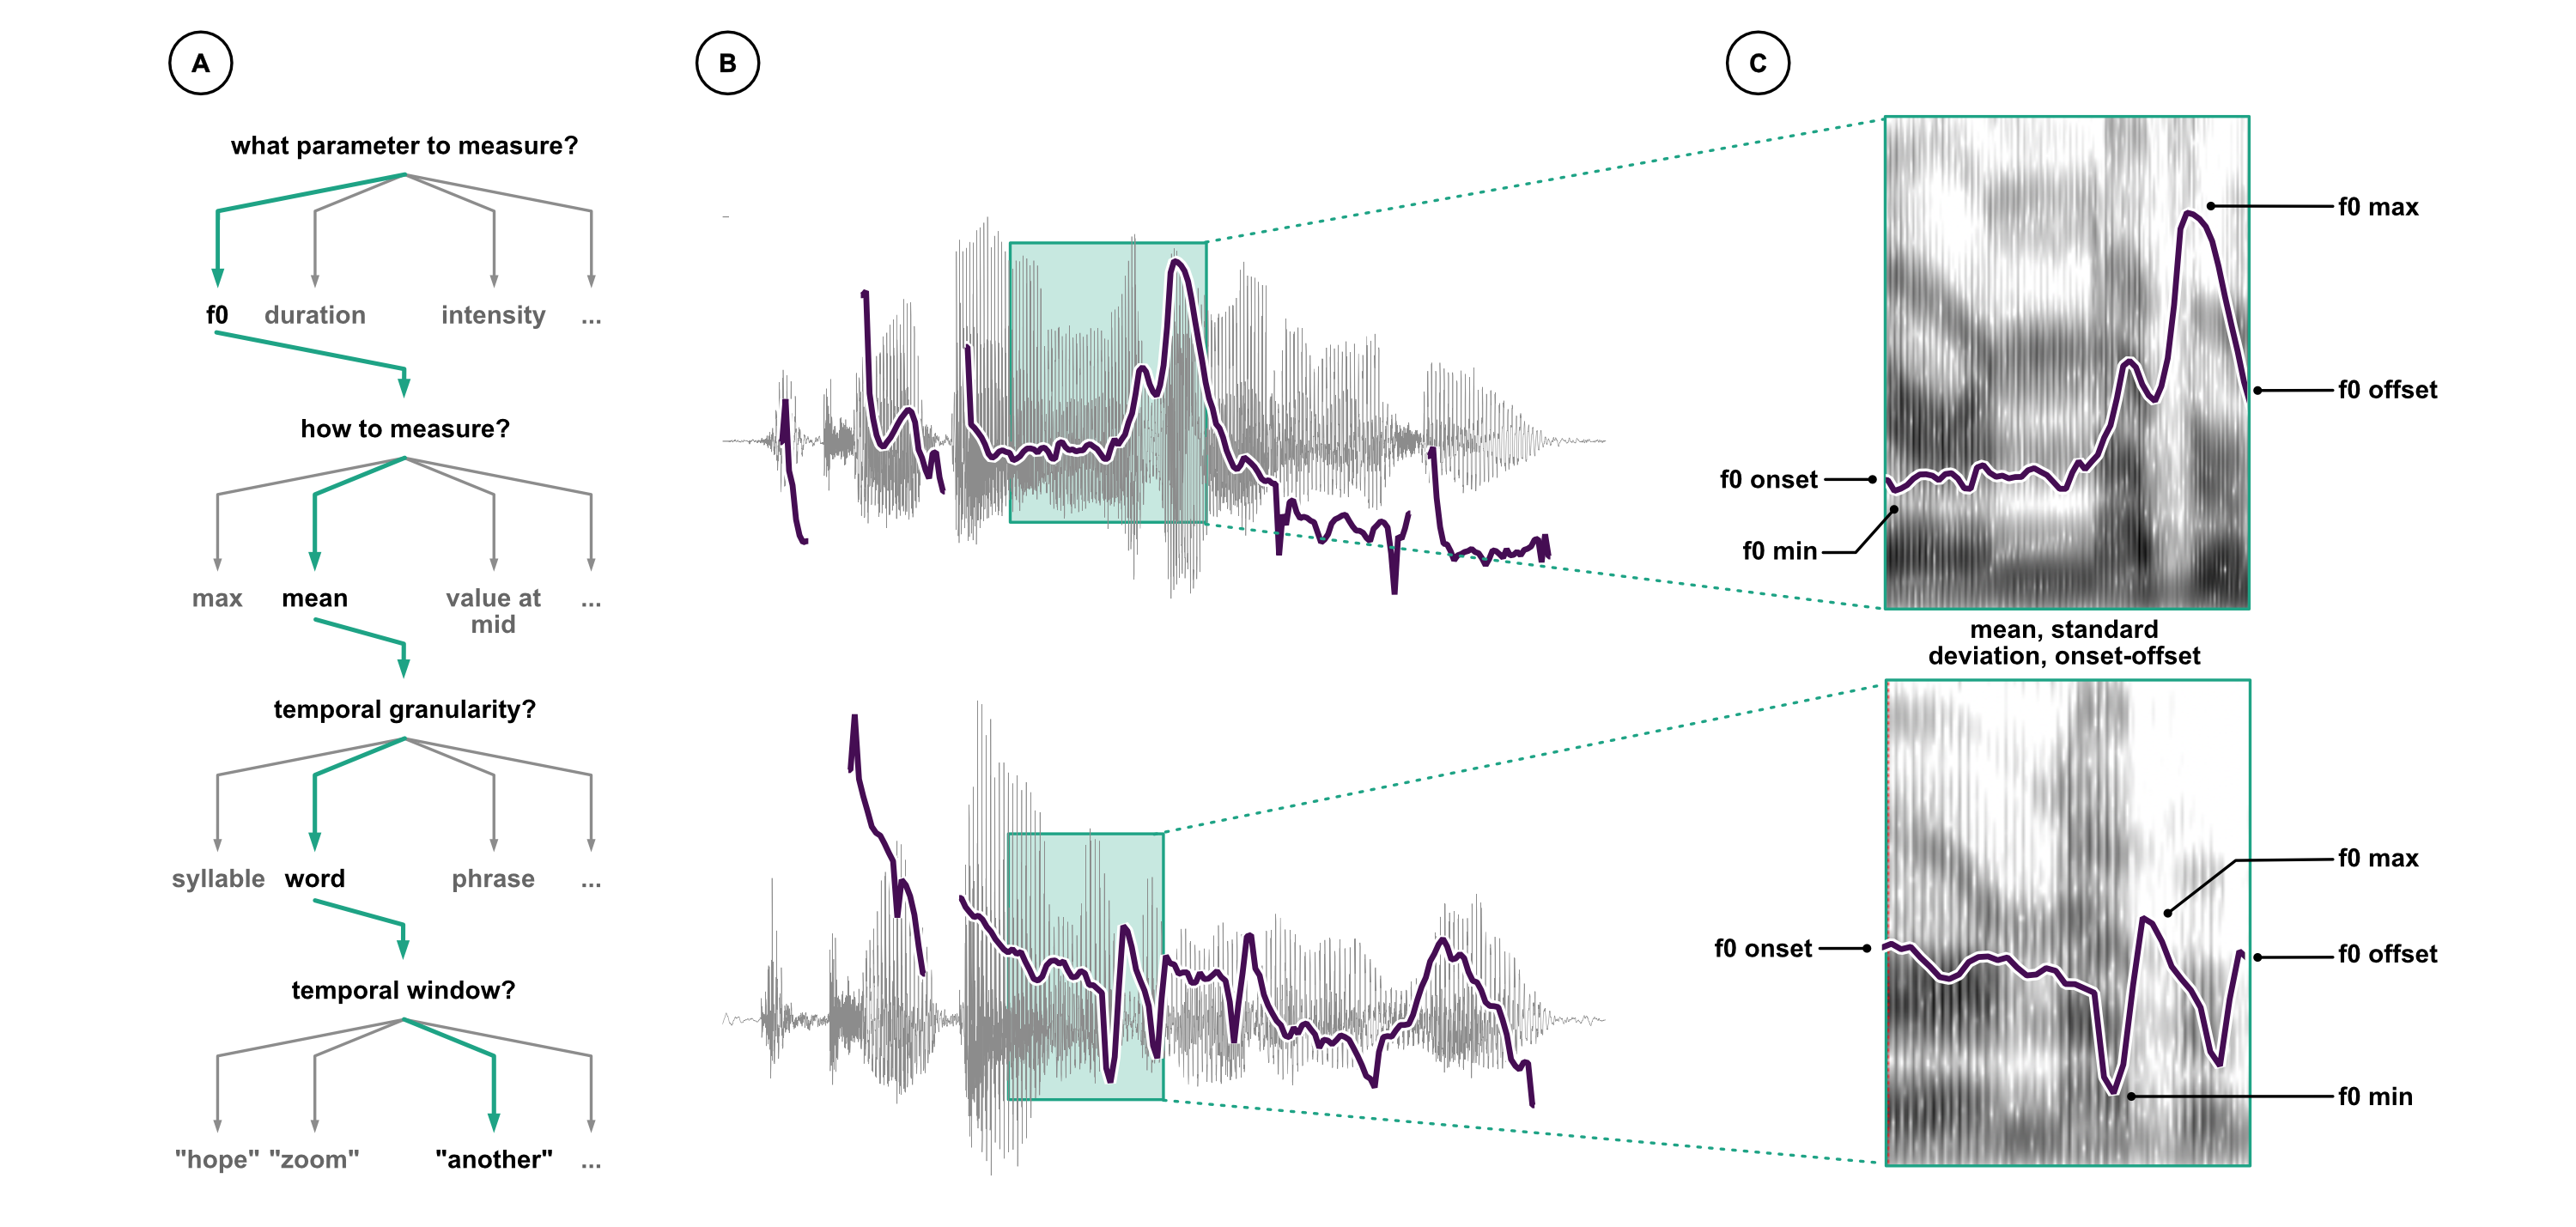
\includegraphics[width=1\linewidth]{../figs/ForkingPaths} \caption{Illustration of the analytic flexibility associated with acoustic analyses. (A) An example of multiple possible and justifiable decisions when comparing two utterances; (B) Waveform and fundamental frequency (f0) track of the utterances \emph{I can't bear ANOTHER meeting on Zoom} and \emph{I can't bear another meeting on ZOOM}. The green boxes mark the word \emph{another} in both sentences; (C) Spectrogram and f0 track of the word \emph{another}, exemplifying possible operationalizations of differences in f0.}\label{fig:forkingPaths}
\end{figure}

When looking at phrase-level temporal domains, the number of alternative analytic pipelines increases substantially.
Figure \ref{fig:forkingPaths}A shows a typical example of a decision tree with which speech researchers are often confronted.
Each of the four analytic decisions in the example have different possible options.
Here only one particular path has been taken. A different one would likely produce different results and might lead to different conclusions.
Once we have decided to compare fundamental frequency of the word \emph{another} across the two utterances, there are still many choices to be made, all of which need to be justified.
As Figures \ref{fig:forkingPaths}B-C illustrate, we could measure f0 at specific points in time like the onset of the temporal window, the offset, or the midpoint.
We could also measure the value or time of the minimum or maximum f0 value.
We could summarize f0 across the entire window and extract the mean, median or standard deviation of f0, all of which have been used to analyze speech data in previous work \citep[see][]{gordon2017acoustic}.
But the journey in the garden of analytic paths goes on.
Other important operationalization steps could involve filtering the audio signal, smoothing the extracted f0 track, removing values that substantially deviate from surrounding values or expectations, either manually or automatically, and so on.

These decisions are intended to be made prior to any statistical analysis, but are at times revised a posteriori in light of unforeseen or surprising outcomes (i.e.~after data collection and/or preliminary analyses).
These myriads of possible decisions are multiplied by those researcher degrees of freedom related to statistical analysis \citep[e.g.][]{wicherts2016}.

In sum, speech data is made of complex physical signals that generates an as-of-yet unappreciated amount of analytic flexibility in the choice of measures and operationalizations.
The present paper probes this garden of forking paths in the analysis of speech.
To assess the variability in data analysis pipelines, including both operationalization and statistical analysis, across independent researchers, we provide analytic teams with an experimentally elicited speech production data set.
The data set derives from the unpublished research project \emph{Prosodic encoding of redundant referring expressions}, which set out to investigate whether speakers acoustically modify utterances to signal unexpected referring expressions.\footnote{Results of this research project were neither published nor publicly presented and are stored on a private OSF repository.}
In the following section we introduce the research question and the experimental procedure of said project, and we describe the resulting data set as used in the current study.

\hypertarget{s:dataset}{%
\subsection{The data set: The acoustic properties of atypical modifiers}\label{s:dataset}}

Referring is one of the most basic and prevalent uses of language and one of the most widely researched areas in language science.
When trying to refer to a banana, what does a speaker say and how do they say it in a given context.
The context within which an entity occurs (i.e., with other non-fruits, other fruits, or other bananas) plays a large part in determining the choice of referring expressions.
Generally, speakers aim to be as informative as possible to uniquely establish reference to the intended object, but they are also resource-efficient in that they avoid redundancy \citep{grice1975logic}.
Thus one would expect the use of a modifier, for example, only if it is necessary for disambiguation.
For instance, one might use the adjective \emph{yellow} to describe a banana in a situation in which there are a yellow and a less ripe green banana available, but not when there is only one banana to begin with.

Despite the coherent idea that speakers are both rational and efficient, there is much evidence that speakers are often over-informative.
Speakers use referring expressions that are more specific than strictly necessary for the unambiguous identification of the intended referent \citep{sedivy2003pragmatic, westerbeek2015stored, rubio2016redundant}, which has been argued to facilitate object identification and make communication between speakers and listeners more efficient \citep{arts2011overspecification, paraboni2007generating, rubio2016redundant}.
Recent findings suggest that the utility of a referring expression depends on how good it is for a listener (compared to other referring expressions) to identify a target object.
For example, \citet{degen2020redundancy} showed that modifiers that are less typical for a given referent (e.g.~a blue banana) are more likely to be used in an over-informative scenario (e.g.~when there is just one banana).
This account, however, has mainly focused on content selection \citep{gatt2013we}, i.e.~what words to use.

Even when morphosyntactically identical expressions are involved, speakers can modulate utterances via suprasegmental acoustic properties like temporal and spectral modifications \citep[e.g.,][]{ladd2008intonational}.
Most prominently, languages can use intonation to signal discourse relationships between referents.
Intonation marks discourse-relevant referents for being new or given information, to guide the listeners' interpretation of incoming messages.
Beyond structuring information relative to the discourse, a few studies suggested that speakers might use intonation to signal atypical lexical combinations \citep[e.g.][]{dimitrova2008prosodic, dimitrova2009did}.
Referential expressions such as \emph{blue banana} were produced with greater prosodic prominence than more typical referents such as \emph{yellow banana}.
These results are in line with the idea of resource-efficient, rational language users who modulate their speech in order to facilitate listeners' comprehension.
However, the above studies are based on a small sample size (10 participants) and on potentially anti-conservative statistical analyses, leaving reason to doubt the generalizability of the studies' conclusions.

To further illuminate the question of whether speakers modify speech to signal atypical referents, and overcome some of the limitations of previous work, thirty native German speakers were recorded in a production study while interacting with a confederate (one of the experimenters) in a referential game, following experimental procedures typical of the field.
The participants had to verbally instruct the confederate to select a specified target object out of four objects presented on a screen.
The subject and confederate were seated at the opposite sides of a table, each facing one of two computer screens.
The participant and the experimenter could not see each other nor each others' screens.
Figure \ref{fig:procedural} shows the experimental procedure time-line.
After a familiarization phase, the subject first saw four colored objects in the top left, top right, bottom left, and bottom right corners of the screen.
One of the objects served as the target, another as the competitor, and the remaining two objects served as distractors.
Objects were referred to using noun phrases consisting of an adjective modifier denoting color and a modified object (e.g.~\emph{Gelbe Zitrone} `yellow lemon', \emph{Rote Gurke} `red cucumber', \emph{Rote Socken} `red socks').



\begin{figure}
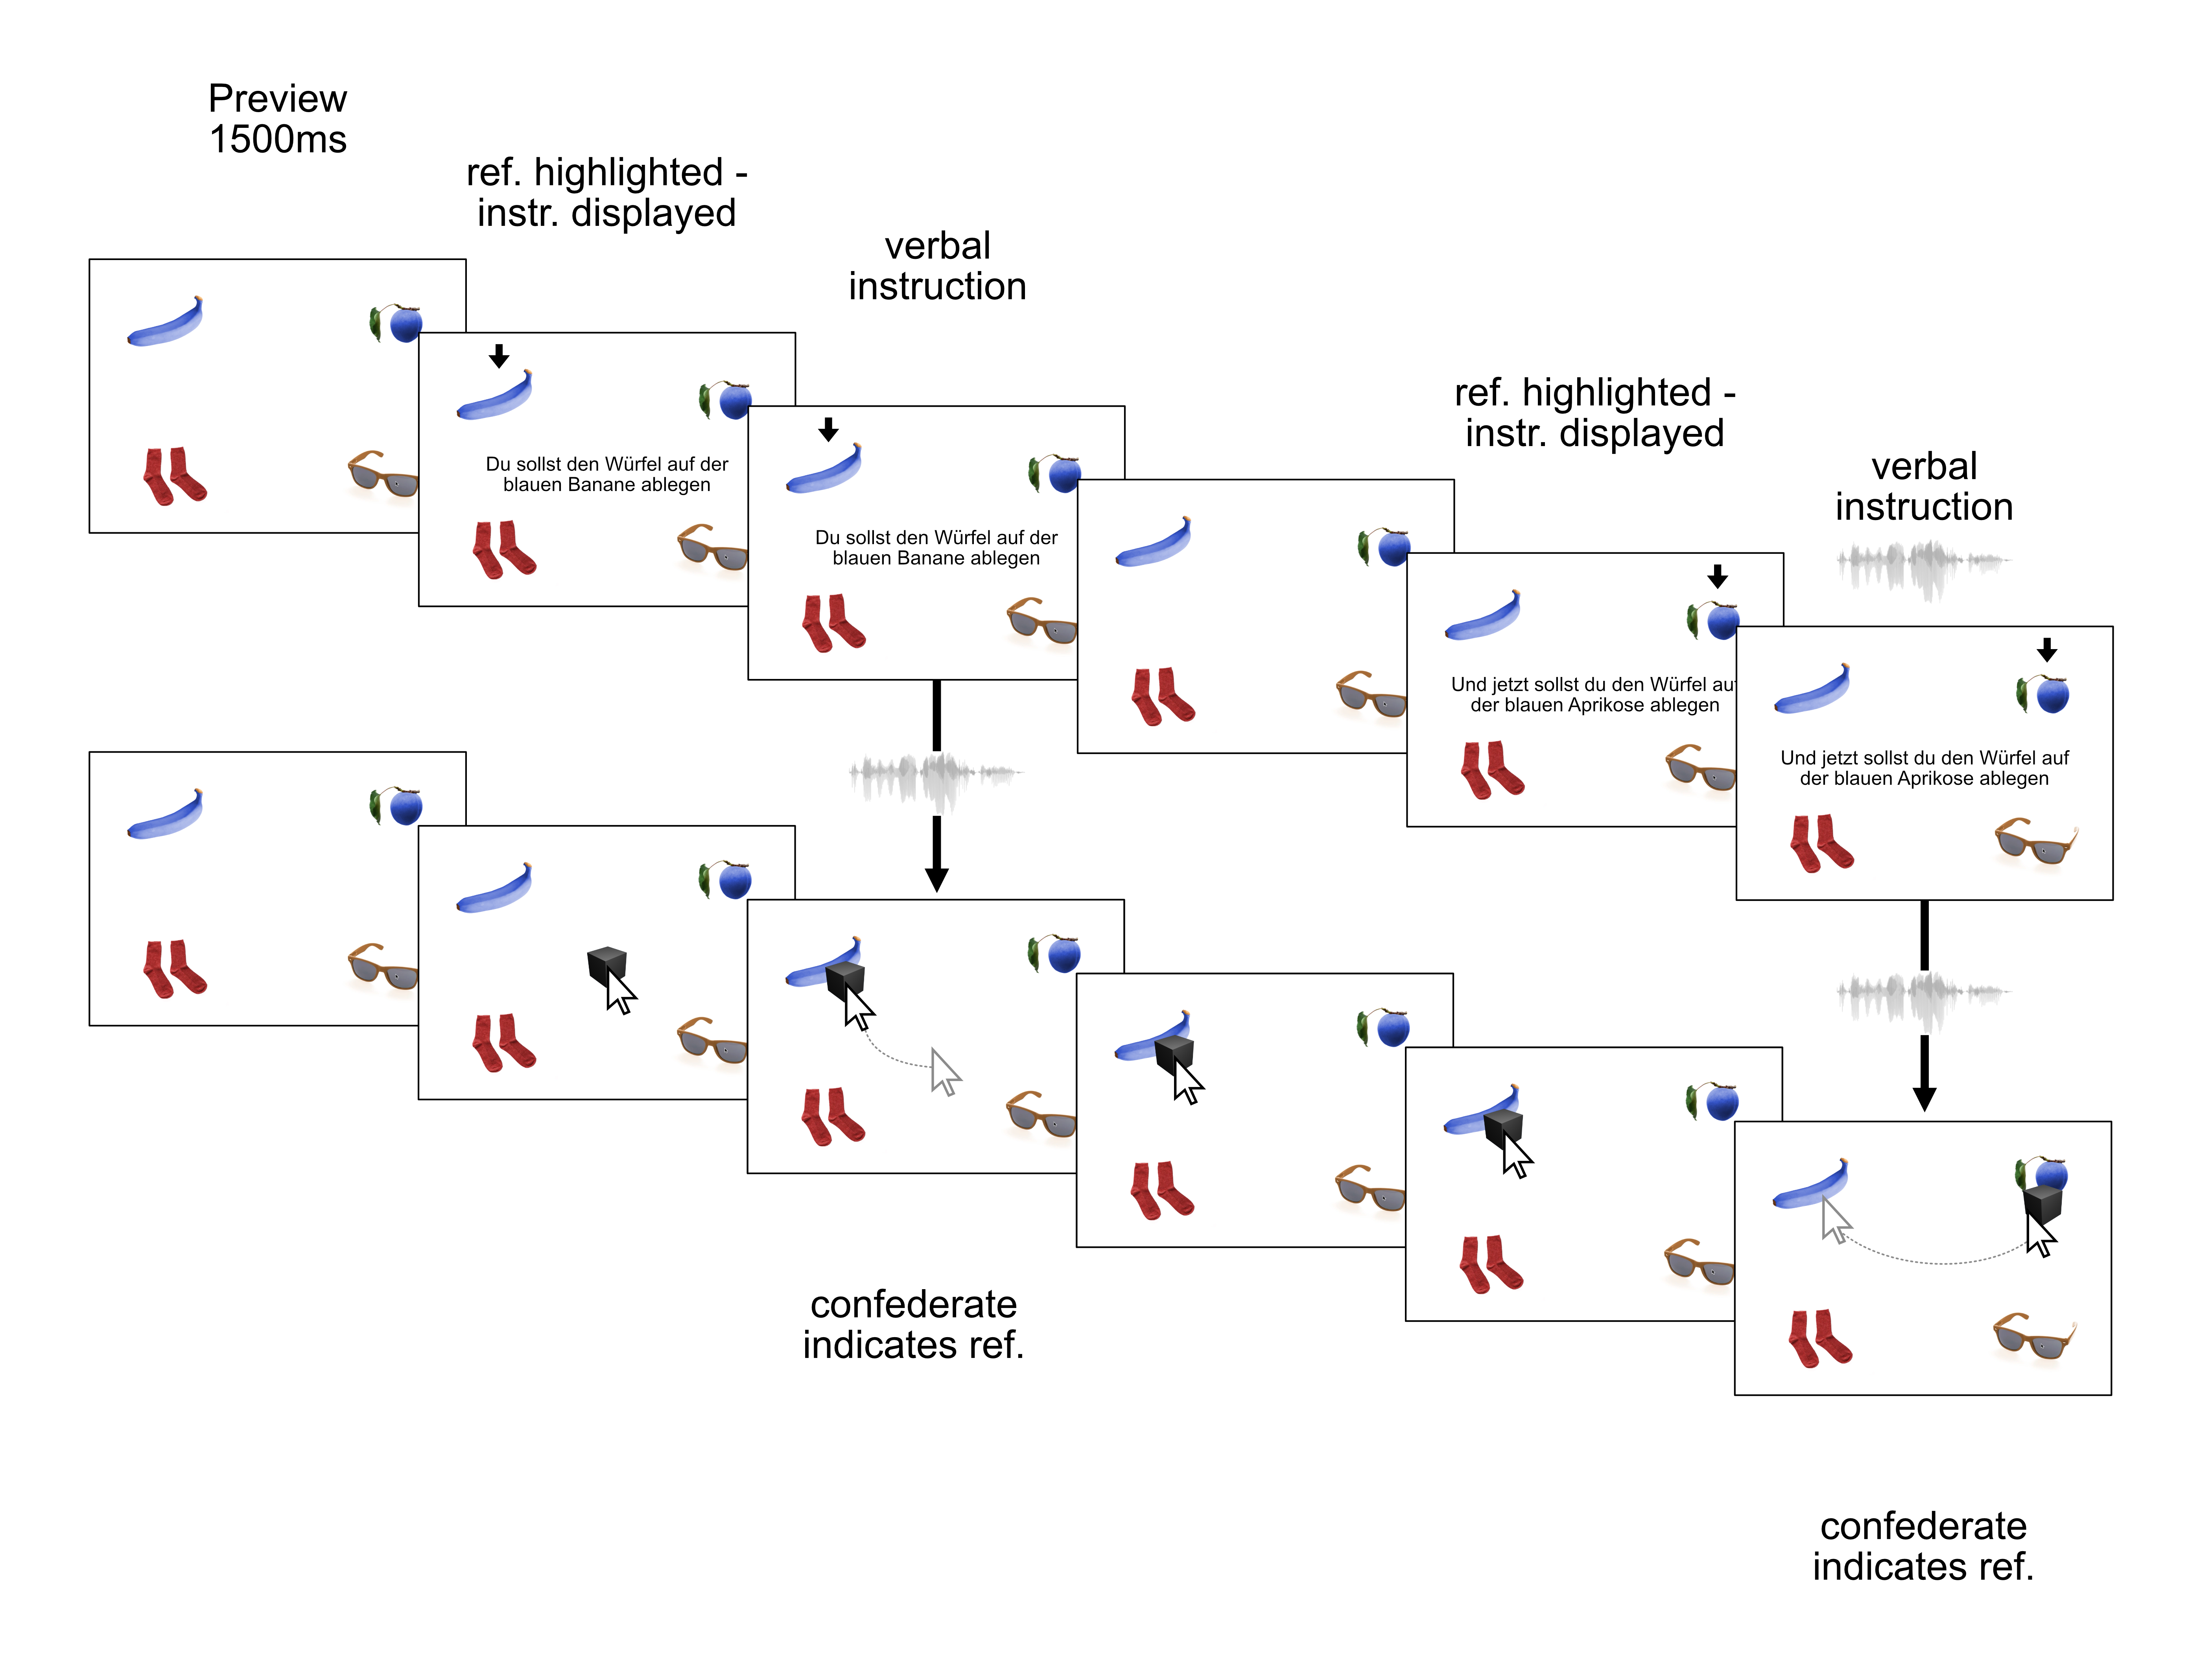
\includegraphics[width=1\linewidth]{../figs/procedure_plot} \caption{Experimental procedure. The upper row illustrates the trial sequence for the speaker (participant) and the lower row illustrates the trial sequence for the confederate. After a preview of 1500ms the speaker sees an arrow indicating one of the referent (b). Reading the orthographic instructions out loud, the speaker gives the confederate verbal instructions onto which referent they should drag the cube (c). The confederate, in turn, drags the black cube onto the target referent (d). Both the arrow and the orthographic instruction disappear from the speaker's screen and a new referent is indicated by an arrow on the same display alongside a new orthographic instruction (e). The speaker gives the confederate verbal instructions (f) which the confederate follows by dragging the cube onto the next referent (g).}\label{fig:procedural}
\end{figure}

In the center of the screen, a black cube was displayed, which could be moved by the experimenter.
The participant would read a sentence prompt out loud (\emph{Du sollst den Würfel auf der COLOR OBJECT ablegen} `You have to put the cube on top of the COLOR OBJECT') to instruct the experimenter to drag the cube on top of one of the four depicted objects (the \emph{competitor}) using the mouse.
After the experimenter had moved the cube as instructed, the subject would read another sentence prompt (\emph{Und jetzt sollst du den Würfel auf der COLOR OBJECT ablegen} `And now, you have to put the cube on top of the COLOR OBJECT') instructing the experimenter to move the cube on top of a different object (the \emph{target}).
The second utterance in the trial was the critical trial for analysis.

The two sentence prompts were used to create a focus contrast between the competitor and the target object.
Focused units denote the set of all (contextually relevant) alternatives \citep[e.g.][]{rooth1992theory}.
Concretely, a focus contrast marks one of more elements in a sentence as prominent, by different linguistic means depending on the language.
For instance, if the competitor and target objects differ but their color does not (e.g.~\emph{yellow banana} vs \emph{yellow tomato}), the noun is said to be in focus.
We call this the Noun Focus condition, or NF for short.
If the objects are the same but differ in color (e.g.~\emph{yellow banana} vs \emph{blue banana}), the color adjective is in focus (the Adjective Focus condition, AF).
If both the color and the object differ (e.g.~\emph{yellow banana} vs \emph{blue tomato}), then the whole noun phrase is in focus (the Adjective/Noun Focus condition, ANF).
The NF condition constituted the experimentally relevant condition, while the AF and ANF conditions acted as fillers.
Crucially, the color-object combinations in the Noun Focus (NF) condition were manipulated with respect to their typicality.
The combinations were either typical (e.g.~\emph{orange mandarin}), medium typical (e.g.~\emph{green tomato}), or atypical (e.g.~\emph{yellow cherry}), as established by a norming study that was conducted prior to the production experiment just described.\footnote{A detailed description of the norming and production studies from the \emph{Prosodic encoding of redundant referring expressions} project, which was given to the analysts with the data set, can be found in \texttt{methods\_norm\_prod.pdf} at \url{https://bit.ly/3Ahawc7}.}
Each subject produced 15 critical trials (NF condition).
Each trial was repeated twice, yielding a total of 30 trials per participant and a grand-total of 900 (\(15 \times 2 \times 30\) participants) spoken utterances.

For the present study, N analysis teams will receive access to the entire data set generated by the production study.
The data set is constituted by audio recordings and annotation files in a format that is typical for the field.
The teams will be instructed to answer the following research question, using the provided data set: \emph{Do speakers acoustically modify utterances to signal atypical word combinations?}

\hypertarget{methods}{%
\section{Methods}\label{methods}}

As outlined in Section \protect\hyperlink{s:operspeech}{Operationalizing speech}, researchers are faced with a large amount of analytic choices when analyzing a multidimensional signal such as speech.
Analysts must identify and operationalize relevant measurements, as well as the temporal domain(s) from which these measurements are to be taken, and then possibly transform said measurements before submitting them to statistical models, which must be chosen alongside inferential criteria.
The complexity of speech data constitutes the ideal testing ground to assess the upper bound of analytic flexibility that social science might face across disciplines.
We will employ a meta-analytic approach to assess (i) the variability of the reported effects, and (ii) how analytic and researcher-related predictors affect the final results.

In this study, we will follow the procedures proposed by \citet{Parker2020} and \citet{aczel2021}.
The project involves the following five phases:

\begin{enumerate}
\def\labelenumi{\arabic{enumi}.}
\tightlist
\item
  \textsc{Recruitment}: We will recruit independent groups of researchers to analyze the data and review others' data analyses.
\item
  \textsc{Team Analysis}: We will give researchers access to the speech corpus and let them analyze the data as they see fit.
\item
  \textsc{Review}: We will ask reviewers to generate peer-review ratings of the analyses based on methods (not results).
\item
  \textsc{Meta-analysis}: We will evaluate variability among the different analyses and how different predictors affect the outcomes.
\item
  \textsc{Write-up}: We will collaboratively produce the final manuscript.
\end{enumerate}

We estimate that this process, from the time of an in-principle acceptance of this Stage 1 Registered Report to the end of Phase 5, will take nine months.
The factor most likely to delay our time-line is the rate of completion of the original set of analyses by independent analysis teams.

The project OSF repository contains all the materials mentioned in this paper and can be accessed at \url{https://bit.ly/3AqU1ul}.
The main repository holds three OSF components, \texttt{Data}, \texttt{Questionnaires}, and \texttt{Cache}, and it is linked to the GitHub repository.
The following sections report the criteria for sample size, data exclusions, data manipulations, and all the measures in the study.

\hypertarget{phase-1-recruitment-of-analysts-and-initial-survey}{%
\subsection{Phase 1: Recruitment of analysts and initial survey}\label{phase-1-recruitment-of-analysts-and-initial-survey}}

An online landing page will provide a general description of the project, including a short pre-recorded slide-show that summarizes the data set and research question (\url{https://many-speech-analyses.github.io}).\footnote{``Questions'' and ``Join Project'' buttons will be functioning when recruitment starts. ``Join Project'' will link to the intake form.}
The project will be advertised via social media, using mailing lists for linguistic and psychological societies, and via word of mouth.
Social media advertising will be accompanied by a short recruitment form (\texttt{recruitment\_form.pdf})
The target population comprises active speech science researchers with a graduate/doctoral degree (or currently studying for a graduate/doctoral degree) in relevant disciplines.
All individuals interested in participating will be asked to complete a questionnaire detailing their familiarity with numerous analytical approaches common in the speech sciences (\texttt{analytic\_approach\_quest.pdf}).
Researchers can choose to work independently or in a small team.
For the sake of simplicity, we will refer both to a single researcher and teams as \textsc{analysis teams}.\footnote{Terms in small caps in this and later sections are included with their definition in the glossary at the end of the paper for the reader's convenience.}
Recruitment for this project will commence upon receiving in-principle acceptance.

As outlined above, our primary aim is to assess the variability of the reported effects, rather than the meta-analytic estimate of the investigated effect \emph{per se}.
To estimate the degree of uncertainty around effect variability as driven by number of teams, we ran a series of sample size simulations with values of variability extracted from \citet{silberzahn2018many}.
The code is available at \url{https://many-speech-analyses.github.io/suppl/simulations.html}, Section 2.\footnote{Cached model outputs can be found at \url{https://bit.ly/3AgdHAN}.}
Variability among teams was operationalized as the standard deviation of the teams' reported effects from \citet{silberzahn2018many} (which we \emph{z}-scored prior to simulations to make it comparable to our study).
For the mean of the teams' true standard deviation (0.68 \emph{z}-score), the simulation indicates that the degree of uncertainty around the estimated teams' standard deviation will be below 1 SD at any sample size greater than 10 teams.
Thus in order to achieve our main goal, i.e.~estimating variability among teams, we consider a minimum sample size of 10 teams as sufficient.
Given the exploratory nature of our study, however, we will sample as many analysts as possible.
We have received initial expression of interest to participate from more than 200 analysts.

After submitting their analyses, we will ask analysts to also function as peer-reviewers. Each team must review four other analyses.
All analysts will share co-authorship on this manuscript and will participate in the collaborative process of producing the final manuscript.
Informed consent will be obtained as part of the intake form.

\hypertarget{phase-2-primary-data-analyses}{%
\subsection{Phase 2: Primary Data Analyses}\label{phase-2-primary-data-analyses}}

The analysis teams will register for participation and each of the analysts individually will answer a demographic and expertise questionnaire (\texttt{intake\_form.pdf}).
A PDF version of this and all other questionnaires are available in the repository's \texttt{Questionnaires} component, at \url{https://bit.ly/3Cf3fdm}.
The questionnaire collects information on the analysts current position and self-estimated breadth and level of statistical expertise and acoustic analysis skills.
We will then request that they answer the question: \emph{Do speakers acoustically modify utterances to signal atypical word combinations?}
To do so, they will be given the data generated by the experiment described in Section \protect\hyperlink{s:dataset}{The data set}.
The data will include the audio recordings with corresponding time-aligned transcriptions in the form of Praat TextGrid files.
These can be found in the \texttt{Data} component at \url{https://bit.ly/3Ahawc7}.

Once their analysis is complete, they will answer a structured questionnaire (\texttt{analytic\_quest.pdf}), providing information about their analysis technique, an explanation of their analytic choices, their quantitative results, and a statement describing their conclusions.
They will also upload their analysis files (including the additionally derived data and text files that were used to extract and pre-process the acoustic data), their analysis code (if applicable), and a detailed journal-ready analysis section.

\hypertarget{phase-3-peer-review-of-analyses}{%
\subsection{Phase 3: Peer Review of Analyses}\label{phase-3-peer-review-of-analyses}}

Each analysis will be evaluated by four different analysts teams who function as peer-reviewers.
Each peer-reviewer will be randomly assigned to analyses from at least four analysis teams.
Reviewers will evaluate the methods of each of their assigned analyses one at a time in a sequence determined by the initiating authors.
The sequences will be systematically assigned so that, if possible, each analysis is allocated to each position in the sequence for at least one reviewer.

The process for a single reviewer will be as follows.
First, the reviewer will receive a description of the methods of a single analysis.
This will include the narrative methods section, the analysis team's answers to the questionnaire regarding their methods, including analysis code and the data set.
The reviewer will then be asked in an online questionnaire (\texttt{peer\_review\_quest.pdf}) to rate both the acoustic and the statistical analyses and to provide an overall rating, using a scale of 0-100, respectively.
To help reviewers calibrate their rating, they will be given the following guidelines:

\begin{itemize}
\item
  \begin{enumerate}
  \def\labelenumi{\arabic{enumi}.}
  \setcounter{enumi}{99}
  \tightlist
  \item
    A perfect analysis with no conceivable improvements from the reviewer.
  \end{enumerate}
\item
  \begin{enumerate}
  \def\labelenumi{\arabic{enumi}.}
  \setcounter{enumi}{74}
  \tightlist
  \item
    An imperfect analysis but the needed changes are unlikely to dramatically alter final interpretation.
  \end{enumerate}
\item
  \begin{enumerate}
  \def\labelenumi{\arabic{enumi}.}
  \setcounter{enumi}{49}
  \tightlist
  \item
    A flawed analysis likely to produce either an unreliable estimate of the relationship or an over-precise estimate of uncertainty.
  \end{enumerate}
\item
  \begin{enumerate}
  \def\labelenumi{\arabic{enumi}.}
  \setcounter{enumi}{24}
  \tightlist
  \item
    A flawed analysis likely to produce an unreliable estimate of the relationship and an over-precise estimate of uncertainty.
  \end{enumerate}
\item
  \begin{enumerate}
  \def\labelenumi{\arabic{enumi}.}
  \setcounter{enumi}{-1}
  \tightlist
  \item
    A dangerously misleading analysis, certain to produce both an estimate that is wrong and a substantially over-precise estimate of uncertainty that places undue confidence in the incorrect estimate.
  \end{enumerate}
\end{itemize}

The reviewers will also be given the option to include further comments in a text box for each of the three ratings.

After submitting the review, a methods section from a second analysis will then be made available to the reviewer.
This same sequence will be followed until all analyses allocated to a given reviewer have been provided and reviewed.
After providing the final review, the reviewer will be simultaneously presented with all four (or more) methods sections that the reviewer has just completed reviewing, the option to revise their original ratings, and a text box to provide an explanation.

\hypertarget{phase-4-evaluating-variation}{%
\subsection{Phase 4: Evaluating variation}\label{phase-4-evaluating-variation}}

The initiating authors (SC, JC, TR) will conduct the analyses outlined in this section.
We will not conduct confirmatory tests of any a priori hypotheses.
We consider our analysis exploratory.

\hypertarget{descriptive-statistics}{%
\subsubsection{Descriptive statistics}\label{descriptive-statistics}}

We will calculate summary statistics describing variation among analyses, including (a) the nature and number of acoustic measures (e.g.~f0 or duration), (b) the operationalization and the temporal domain of measurement (e.g.~mean of an interval or value at specified point in time), (c) the nature and number of model parameters for both fixed and random effects (if applicable), (d) the nature and reasoning behind inferential assessments (e.g.~dichotomous decision based on \emph{p}-values, ordinal decision based on a Bayes factor), as well as the (e) mean, (f) standard deviation and (g) range of the standardized effect sizes (see the next section for the standardization procedure).

\hypertarget{s:meta-est}{%
\subsubsection{Meta-analytic estimation}\label{s:meta-est}}

We will investigate the variability in \textsc{reported effect sizes} using Bayesian meta-analytic techniques.
As the measure of variability, we will take the meta-analytic \textsc{group-level standard deviation} (\(\sigma_{\alpha_{\text{t}}}\), see below), where the groups are the analysis teams.

Based on the common practices currently in place within the field, we anticipate that researchers will use multilevel regression models, thus common measurements of effect size, such as Cohen's \(d\), may be inappropriate.
Furthermore, \citet{aczel2021} suggest that directly asking analysts to report standardized effect sizes could bias the choice of analyses towards types that more straightforwardly return a standardized effect.
Since the variables used by the analysis teams might substantially differ in their measurement scales (e.g, Hertz for frequency vs milliseconds for duration), we will standardize all reported effects by refitting each \textsc{reported model} with centered and scaled continuous variables (\emph{z}-scores, i.e.~the observed values subtracted from the mean divided by the standard deviation) and sum-coded factor variables.
Factor-level ordering for each categorical variable will mirror that of the original analyses.
Each \textsc{standardized model} will be fitted as a Bayesian regression model with Stan \citep{stan2021}, RStan \citep{stan2020a}, and brms \citep{burkner2017} in R \citep{R-base}.
For those reported models that were originally fitted within a frequentist approach, uniform distributions will be used as the priors of all parameters (with the restriction that only positive numbers will be included for scale parameters), to approximate the estimation procedure of frequentist models (i.e.~only the distribution of the data determines the posterior distribution).
If a team has fitted Bayesian models, the same priors as reported by the team will be used in fitting the respective standardized model.
Model refitting will also constitute a way of validating the reported analyses, a step recommended by \citet{aczel2021}.

The coefficients of the critical predictors (i.e.~critical according to the analysis teams' self-reported inferential criteria) obtained from the standardized models will be used as the \textsc{standardized effect size} (\(\eta_i\)) of each reported model.
If multiple predictors within a single analysis have been reported as critical, each will be included in the meta-analytic model (described in details in the next paragraph).
Moreover, to account for the differing degree of uncertainty around each standardized effect size, we will use the standard deviation of each standardized effect size as the \textsc{standardized standard error} (\(\text{se}_i\)).
This will enable us to fit a so-called ``measurement-error'' model, in which both the standardized effect sizes and their respective standard errors are entered in the meta-analytic model.
As a desired consequence, effect sizes with a greater standard error will be weighted less than those with a smaller standard error in the meta-analytic calculations.

After having obtained the standardized effect sizes \(\eta_i\) with related standard errors \(\text{se}_i\), for each critical predictor of the individual reported model, we will conduct a \textsc{Bayesian random-effects meta-analysis} using a multilevel (intercept-only) regression model.
The outcome variable will be the set of standardized effect sizes \(\eta_i\).
The likelihood of \(\eta_i\) is assumed to correspond to a normal distribution \citep{knight2000}.
The analysis teams will be entered as a group-level effect (i.e., \texttt{(1\ \textbar{}\ team)}, called \emph{random effect} in the frequentist literature).
The standard errors \(\text{se}_i\) will be included as the standard deviation of \(\eta_i\) to fit a measurement-error model, as discussed above.
We will use regularizing weakly-informative priors for the intercept \(\alpha\) (\(Normal(0, 1)\)) and for the group-level standard deviation \(\sigma_{\alpha_{\text{t}}}\) (\(HalfCauchy(0, 1)\)).
We will fit this model with 4 chains of Hamiltonian Monte-Carlo sampling for the estimation of the joint posterior distribution, using the No U-Turn Sampler (NUTS) as implemented in Stan \citep{stan2021}, and 4000 iterations (2000 for warm-up) per chain, distributed across 4 processing cores.
In case of divergent transitions, we will increase \texttt{adapt\_delta}, \texttt{tree\_depth}, and the number of iterations in this order until we obtain a model fit with no divergent transitions.
The code used to run the model can be found at \url{https://many-speech-analyses.github.io/suppl/simulations.html}.

The posterior distribution of the population-level intercept \(\alpha\) will allow us to estimate the range of probable values of the standardized effect size \(\hat{\eta}\).
The posterior distribution will further allow us to investigate the effect of a set of analytic and researcher-related predictors, detailed in the next section.
Crucially, the posterior distribution of the \href{.smallcaps}{group-level standard deviation} \(\sigma_{\alpha_{\text{t}}}\) (i.e.~the standard deviation of the group-level effect of team) will allow us to quantify the degree of variation between the teams' analyses on a standardized scale.

\hypertarget{anares-preds}{%
\subsubsection{Analytic and researcher-related predictors affecting effect sizes}\label{anares-preds}}

As a second step, we will investigate the extent to which the individual standardized effect sizes are affected by a series of \textsc{analytic and researcher-related predictors}.

\textbf{Analytic predictors}. We will estimate the influence of the following predictors related to the analytic characteristics of each team's reported analysis:

\begin{itemize}
\tightlist
\item
  \emph{Measure of uniqueness} of individual analyses for the set of predictors in each model {[}numeric{]}.
\item
  \emph{Measure of conservativeness} of the model specification, as the number of random/group-level effects included {[}numeric{]}.
\item
  \emph{Number of post-hoc changes to the acoustic measurements} the teams will report to have carried out {[}numeric{]}.
\item
  \emph{Number of models} the teams will report to have run {[}numeric{]}.
\item
  \emph{Major dimension} that has been measured to answer the research question {[}categorical{]}.
\item
  \emph{Temporal window} that the measurement is taken over {[}categorical{]}.
\item
  \emph{Average peer-review rating}, as the mean of the overall peer-review ratings for each analysis {[}numeric{]}.
\end{itemize}

Following \citet{Parker2020}, the measure of uniqueness of predictors will be assessed by the Sørensen-Dice Index \citep[SDI,][]{dice1945, sorensen1948}.
The SDI is an index typically used in ecology research to compare species composition across sites.
For our purposes, we will treat predictors as species and individual analyses as sites.
For each pair of analyses \((X, Y)\), the SDI will be obtained using the following formula:

\[\text{SDI} = \frac{2|X \cap Y|}{|X|+|Y|}\]

where \(|X \cap Y|\) is the number of variables common to both models in the pair, and \(|X|+|Y|\) is the sum of the number of variables that occur in each model.

In order to generate a unique SDI for each analysis team, we will calculate the average of all pairwise SDIs for all pairs of analyses using the \texttt{beta.pair()} function in the betapart R package \citep{baselga2020}.

The major measurement dimension of each analysis will be categorized according to the following possible groups: \emph{duration}, \emph{amplitude}, \emph{fundamental frequency}, \emph{other spectral properties} (e.g.~frequency, center of gravity, harmonics difference, etc.), and \emph{other measures} (e.g.~principal components, vowel dispersion, etc.).
The temporal window that the measurement is taken over is defined by the target linguistic unit.
We assume the following relevant linguistic units: \emph{segment}, \emph{syllable}, \emph{word}, \emph{phrase}.
Since each analysis will receive more than one peer-review rating, we will calculate the mean rating and its standard deviation for each.
These will be entered in the model formula as a measurement-error term (\texttt{me(mean,\ sd)} in brms).

\textbf{Researcher-related factors}. We will also include the following predictors:

\begin{itemize}
\tightlist
\item
  \emph{Research experience} as the elapsed time from receiving the PhD. Negative values will indicate that the person is a student or graduate students {[}numeric{]}.
\item
  \emph{Initial belief} in the presence of an effect of atypical noun-adjective pairs on acoustics, as answered during the intake questionnaire {[}numeric{]}.
\end{itemize}

To obtain an aggregated research experience score and initial belief score for each team based on the members' individual scores, we will calculate the mean and standard deviation of these predictors for each team.
These will be entered in the model formula as a measurement-error term (\texttt{me(mean,\ sd)} in brms).
The expedient of using a measurement-error term (which includes the teams' standard deviation) ensures information about within-team variance is not lost (which would be the case if including the mean only).

\textbf{Model specification}. The model will be fitted as a measurement-error model, with the predictors detailed in the preceding paragraphs.
The outcome variable of the model will be the standardized effect sizes and related standard deviation.

A normal distribution will be used as the likelihood function of \(\alpha_{t[i]}\).
The mean of \(\alpha_{t[i]}\) is modeled on the basis of the overall intercept \(\beta\) and on the coefficients of each predictor.
The numeric predictors will be centered and scaled and the categorical predictors will be sum coded.
As the prior for the intercept and the predictors we will use a normal distribution with mean 0 and standard deviation 1.
The model will be run with the same settings as with the meta-analytic model.
The code used to run the model can be found at \url{https://many-speech-analyses.github.io/suppl/simulations.html}.

\hypertarget{ana-archive}{%
\subsubsection{Data management}\label{ana-archive}}

All relevant data, code, and materials will be publicly archived on the Open Science Framework (\url{https://osf.io/3bmcp/}, link for peer-review: \url{https://bit.ly/3AqU1ul}).
Archived data will include the original data set distributed to all analysts, any edited versions of the data analyzed by individual teams, and the data we analyze with our meta-analyses, which include the standardized effect sizes, the statistics describing variation in model structure among analysis teams, and the anonymized answers to our questionnaires of analysts.
Similarly, we will archive both the analysis code used for each individual analysis and the code from our meta-analyses.
We will also archive copies of our survey instruments from analysts and peer-reviewers.

We will exclude from our synthesis any individual analysis submitted after we have completed peer review or those unaccompanied by analysis files that allow us to understand what the analysts did.
We will also exclude any individual analysis that does not produce an outcome that can be interpreted as an answer to our primary question.

\hypertarget{phase-5-collaborative-write-up-of-manuscript}{%
\subsection{Phase 5: Collaborative Write-Up of Manuscript}\label{phase-5-collaborative-write-up-of-manuscript}}

Analysts and initiating authors will discuss the limitations, results, and implications of the study and collaborate on writing the final manuscript for review as a stage-2 Registered Report.

\hypertarget{results}{%
\section{Results}\label{results}}

The results section is divided into three parts.
We first provide a statistical description of team composition, nature of acoustic analyses and statistical approaches, and peer-review ratings of these two as obtained by the team members.
Second, we report the results of the meta-analytic model, focussing on between-team variability and the estimated meta-analytic effect of word combination typicality on speech acoustics.
Finally, we present the analysis of the effect of analytic and researcher-related predictors on the meta-analytic effect.

\hypertarget{descriptive-statistics-1}{%
\subsection{Descriptive statistics}\label{descriptive-statistics-1}}

In the following sections, we will describe the characteristics of the analysis teams that participated in the study and the analytic approaches they adopted.
An important aspect that emerges from the descriptive analysis is the large variation in analytic strategies.

\hypertarget{characteristics-of-analytic-teams}{%
\subsubsection{Characteristics of analytic teams}\label{characteristics-of-analytic-teams}}

Eighty-Four teams initially signed up to participate in the study.
Fifty-Four of the signed-up teams dropped out during the analysis phase\footnote{ADD REASONS}.
The remaining 30 teams submitted their analysis by the established deadline.
These are the teams that are included in this study.

Submitting teams consisted of an average of 3.63 individual analysts (SD = 2.8).

Upon sign-up, we collected background information from each analyst through the intake form, which was administered during Phase 1, prior to the distribution of the data to the teams.
Analysts had on average 4.8 years (SD = 4.2) of experience after completing their PhD, ranging from -3.8 years, i.e.~PhD students (or younger) to 12.4 years.
The analysts' prior belief in the effect under investigation on a scale from 0 to 100 ranged from 48.5 to 92 with an average of 69.2 (SD = 11.3).
We take this to suggest that analysts had an overall rather high positive prior belief in the investigated relationship between prosody and word combination typicality.

At the end of Phase 2 (primary data analysis), the teams have submitted a grand total 100 individual models to answer the research question, with a mean of 3.6 models per team.
Crucially, the analytic approaches employed by the teams varied widely both in the acoustical analyses of the speech signal and in the statistical analyses of the obtained measures.
We proceed to discuss these in the following sections, after which we provide an overview of the peer-review ratings.

\hypertarget{acoustic-analysis}{%
\subsubsection{Acoustic analysis}\label{acoustic-analysis}}

The analytic teams differed in their approach to the acoustic analysis of the speech signal, including choosing specific acoustic measures, the temporal window over which they are taken from and how the measures are transformed.
34\% of models used a measure of duration as the outcome variable, 36\% used fundamental frequency (f0), 14\% used vowel formants, 13\% intensity, and 3\% other measures.

45\% of models obtained acoustic measures at the level of the segment (e.g.~comparing the acoustic profile of a vowel), 44\% from the word level (e.g.~comparing the acoustic profile of \emph{Banane} `banana'), 4\% at the level of the phrase (e.g.~the noun phrase including determiner and adjective, e.g.~``the green banana''), 2\% from the whole sentence, and 5\% used a different time window.
Based on a coarse coding of how acoustic measures were operationalized, we find a total of 52 different measurement specifications.

\hypertarget{statistical-analysis}{%
\subsubsection{Statistical analysis}\label{statistical-analysis}}

The high variability of acoustic measurements is multiplied by the choices of statistical analysis, including the chosen inferential framework, the type of model, and the model specification, like choice of predictors, interactions and group-level (aka random) effects.

The models included a mean of 2 different predictors (defined as variables or columns in the data table).
This means that, in addition to the critical predictor (typicality of the adjective noun combinations), there was on average at least an additional predictor.
Among the predictors included in the models there were information structure of the sentence, trial number, semantic dimensions of the referent, part of speech, or speaker gender.

The data given to the teams allowed them to operationalize the predictor of interest, word typicality, in different ways.
Among the possible operationalizations, 79\% of models contained typicality as a categorical variable (e.g.~atypical vs.~typical), 18\% used a continuous typicality scale from 0-100 by calculating the mean typicality for each word combination as obtained from the norming study, while 2\% of the models used the median typicality rating.

The majority of models were run within a frequentist framework (80\%).
20\% were run within a Bayesian framework.
While teams almost exclusively used linear models to analyze their data (98\%, with a few exception using machine learning techniques or GAMs as a special case of linear models), teams differed drastically in how they accounted for dependencies within the data.

The data contains several dependencies between data points, with multiple data points coming from the same subject and with multiple data points being associated with the same adjective or noun.
The appropriate way to account for this non-independence is by using multi-level models and specifying so-called random effects \citep[e.g.,][]{gelman2006data, schielzeth2009conclusions}.
5\% of linear models specified no random effects at all (without pooling their data), so effectively ignoring these non-independences \citep{hurlbert1984pseudoreplication}.
66\% specified random intercepts only, and 29\% specified random intercepts and random slopes to account for the non-independence.
On average, teams that specified random effects, included 2.4 random terms in their models.
Based on statistical framework, type of model, distribution family, fixed terms, and discarding random effects, there were a total of 45 different model specifications.

\hypertarget{review-ratings}{%
\subsubsection{Review ratings}\label{review-ratings}}

Teams reviewed each others' acoustic and statistical analyses.
The mean rating of the acoustic analyses, on a scale from 0 to 100, is 74.5 (SD = 11.2).
The mean rating of the statistical analysis is 73.8 (SD = 14.1).
For reference, as mentioned in the Methods section, a score of 75 was defined as ``an imperfect analysis but the needed changes are unlikely to dramatically alter the final interpretation'', indicating that on average reviewers judged the provided analyses to be appropriate, although ``imperfect''.

\hypertarget{meta-analytic-estimation}{%
\subsection{Meta-analytic estimation}\label{meta-analytic-estimation}}

This section deals with the meta-analytic analysis of the results submitted by the teams.
We first report on the between-team variability estimate, which is the focus of this study, followed by the meta-analytic intercept estimate.

\hypertarget{between-team-variability}{%
\subsubsection{Between-team variability}\label{between-team-variability}}

As explained in the \textbf{Methods} section, the primary aim of this is to assess the variability of the reported effects or, in other words, the degree of between-team variability.
As a measure of between-team variability, we chose to use the meta-analytic group-level standard deviation \(\sigma_{\alpha_{\text{t}}}\)), i.e.~the standard deviation of the group-level effect of team returned by the meta-analytic model.

According to the meta-analytic model, the group-level standard deviation for team is between 0.03 and 0.07 standard units, at 95\% credibility.
This means that the mean deviations of any individual team from the meta-analytic effect estimate range between ±0.06 to ±0.14 (0.3 * 2, 0.07 * 2) in standard units.

\textbf{Non-preregistered}. In our preregistration we did not take into account the possibility that teams might submit multiple analyses/models.
We have run two further non-preregistered meta-analytic models:

\begin{enumerate}
\def\labelenumi{\arabic{enumi}.}
\tightlist
\item
  A model with model ID instead of team as the group-level effect (\texttt{(1\textbar{}model\_id)}).
\item
  A model with team and model ID nested within team as group-level effects (\texttt{(1\textbar{}team)\ +\ (1\textbar{}team:model\_id}).
\end{enumerate}

Based on the first non-preregistered model, the group-level standard deviation for model ID is between 0.11 and 0.15 standard units, at 95\% credibility.
This means that the deviations of any individual analysis model from the meta-analytic effect estimate range between ±0.22 to ±0.3 (0.11 * 2, 0.15 * 2) in standard units.

As for the second non-preregistered model, the posterior estimate for model ID is identical to that of the first non-preregistered model.
On the other hand, the posterior 95\% CrI for team in the second non-preregistered model is 0 and 0.05 standard units (\(\beta\) = 0.02, SD = 0.01), corresponding to a mean deviation range of ±0.1 standard units.

We illustrate what all this means in actual acoustic measures by means of examples, taking the minimum and maximum sample standard deviation of each measure from our data.

\hypertarget{meta-analytic-intercept}{%
\subsubsection{Meta-analytic intercept}\label{meta-analytic-intercept}}

The meta-analytic model estimates the range of probable values of the standardized effect size to be between -0.024 and 0.021 standard units (95\% CrI, mean = -0.001).
In other words, our best guess is that typical and atypical word combinations might not differ in acoustic measures (e.g.~duration, f0 etc,) or, if they do, they do so by a maximum of ±0.02 standard units.

\textbf{Non-preregistered}. As mentioned in the previous section, we have run two further models, one using model ID instead of team and the second using team and model ID nested within team.
In the first model, the meta-analytic intercept estimate is between -0.01 and 0.04 standard units (95\% CrI, mean = 0.015).
This suggests that the acoustic measures of typical word combinations are 0.01 standard units lower to 0.04 standard units higher than the measures of atypical word combinations, at 95\% confidence.
Relative to the preregistered model, this model suggests a somewhat positive effect of typicality (although small negative effects are also possible).
The estimated intercept from the second model (with nested group-level effects) is virtually identical to the first (with only model ID as group-level effect).

(ref:meta\_plot1) illustrates the individual model intercepts, sorted in ascending order based on their mean.
Given the nature and wide variety of acoustic operationalizations, there is not always a natural interpretation of the scale, but in most cases a positive effect corresponds to typical word combinations eliciting higher acoustic values (e.g.~longer duration, higher f0, etc.), as mentioned above.
Notably, while the majority of models yields inconclusive results, there are 27 model estimates for which the 95\% credible interval does not contain zero (16\%).

\begin{figure}
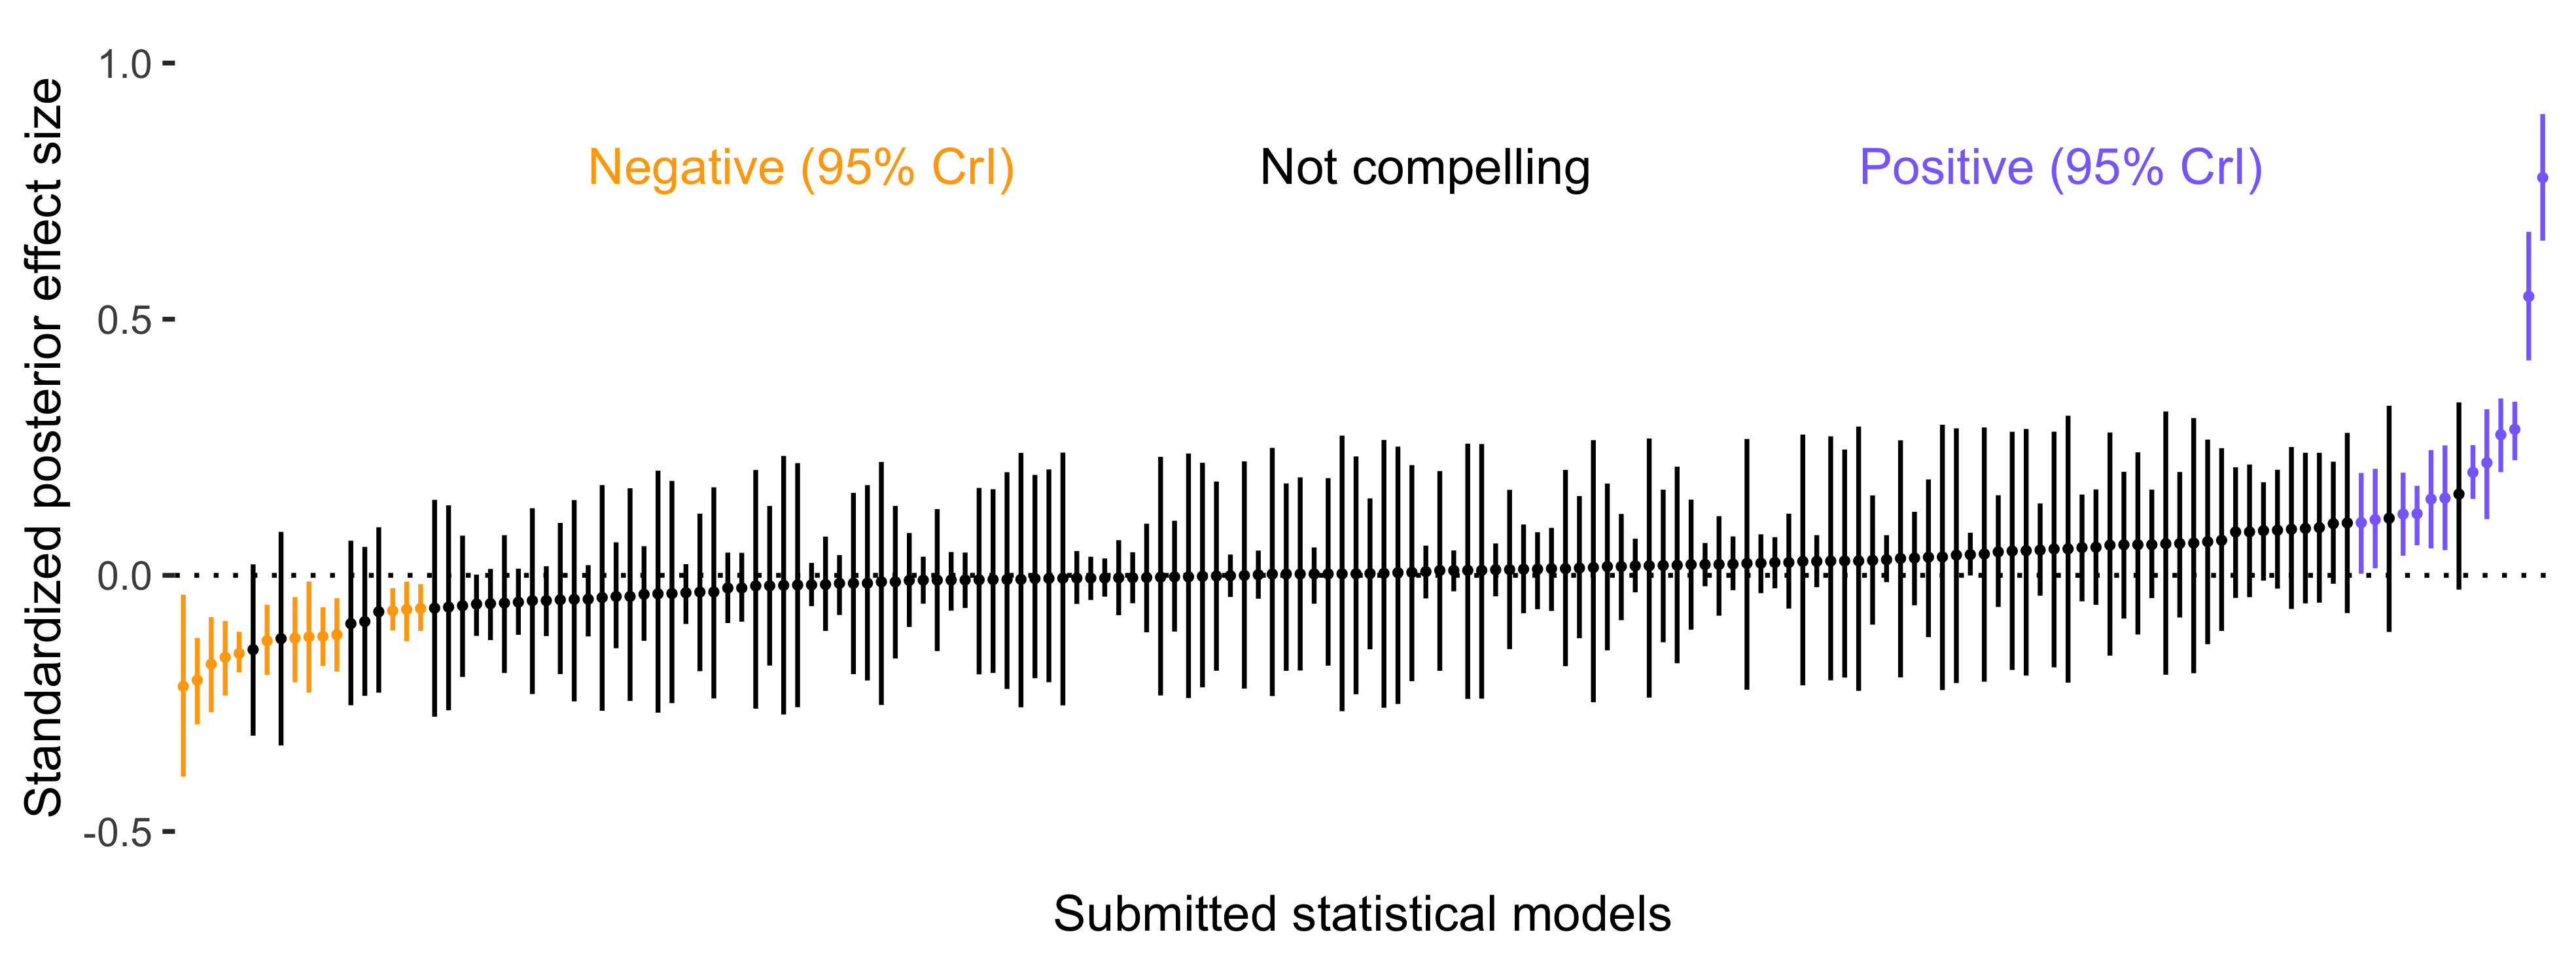
\includegraphics[width=1\linewidth]{../figs/meta_plot1_nest} \caption{(ref:metaPlot1)}\label{fig:plot-meta1}
\end{figure}

\hypertarget{analytic-and-researcher-related-predictors}{%
\subsection{Analytic and researcher-related predictors}\label{analytic-and-researcher-related-predictors}}

After assessing the variability across teams and models, we now turn toward estimating the impact of a series of predictors on the estimated intercept.
There is a lot of variation, raising the question as to whether we can explain some of this variation or whether it is idiosyncratic \citep{breznau2021observing}?

(ref:meta\_plot1), panel C, displays the coefficients alongside 80\% and 95\% credible intervals for all model predictors.

The model suggests that most team-specific predictors yield very small deviations from the meta-analytical estimate and their 95\% credible intervals include zero, leaving us highly uncertain about their direction.
Neither analysts' prior beliefs in the phenomenon (ADD EST + 95CrI), nor their seniority in terms of years after completing their PhD (ADD EST + 95CrI) seem to compellingly affect model estimates.
Similarly, the evaluation of the quality of the analysis from their peers yielded a rather small effect magnitude, again characterized by large uncertainty (ADD EST + 95CrI).
Interestingly, the model uniqueness, i.e.~how unique the choice and combination of predictors is, affects the analysts estimate, with more unique models producing higher positive estimates.
This suggests that the analysts' results very much depend on their choice of predictors.
Looking at the most important choices during measurement, both the acoustic parameter under investigation (e.g.~duration or f0) and the choice of temporal window affected the results.
(ref:meta\_plot1) displays the posterior estimates for the measurement outcome (i.e.~what acoustic dimension was measured, panel A) and measurement window (i.e.~what is the unit over which was measured, panel B).
If an acoustic dimension related to f0 was measured, estimates are lower than the meta analytic estimate.
If on the other hand, vowel formants were measured, estimates are higher than the meta analytic estimate.
Similarly, if acoustic parameters were measured within individual segments (e.g.~the vowel of the noun), estimates are lower than the meta analytic estimate, and if acoustic parameters were measured across whole phrases (e.g.~``the blue banana''), the estimates are generally higher.
In other words, depending on the choice of measurement, analysts arrived at opposite conclusions about how and if typicality is expressed acoustically.

\begin{figure}
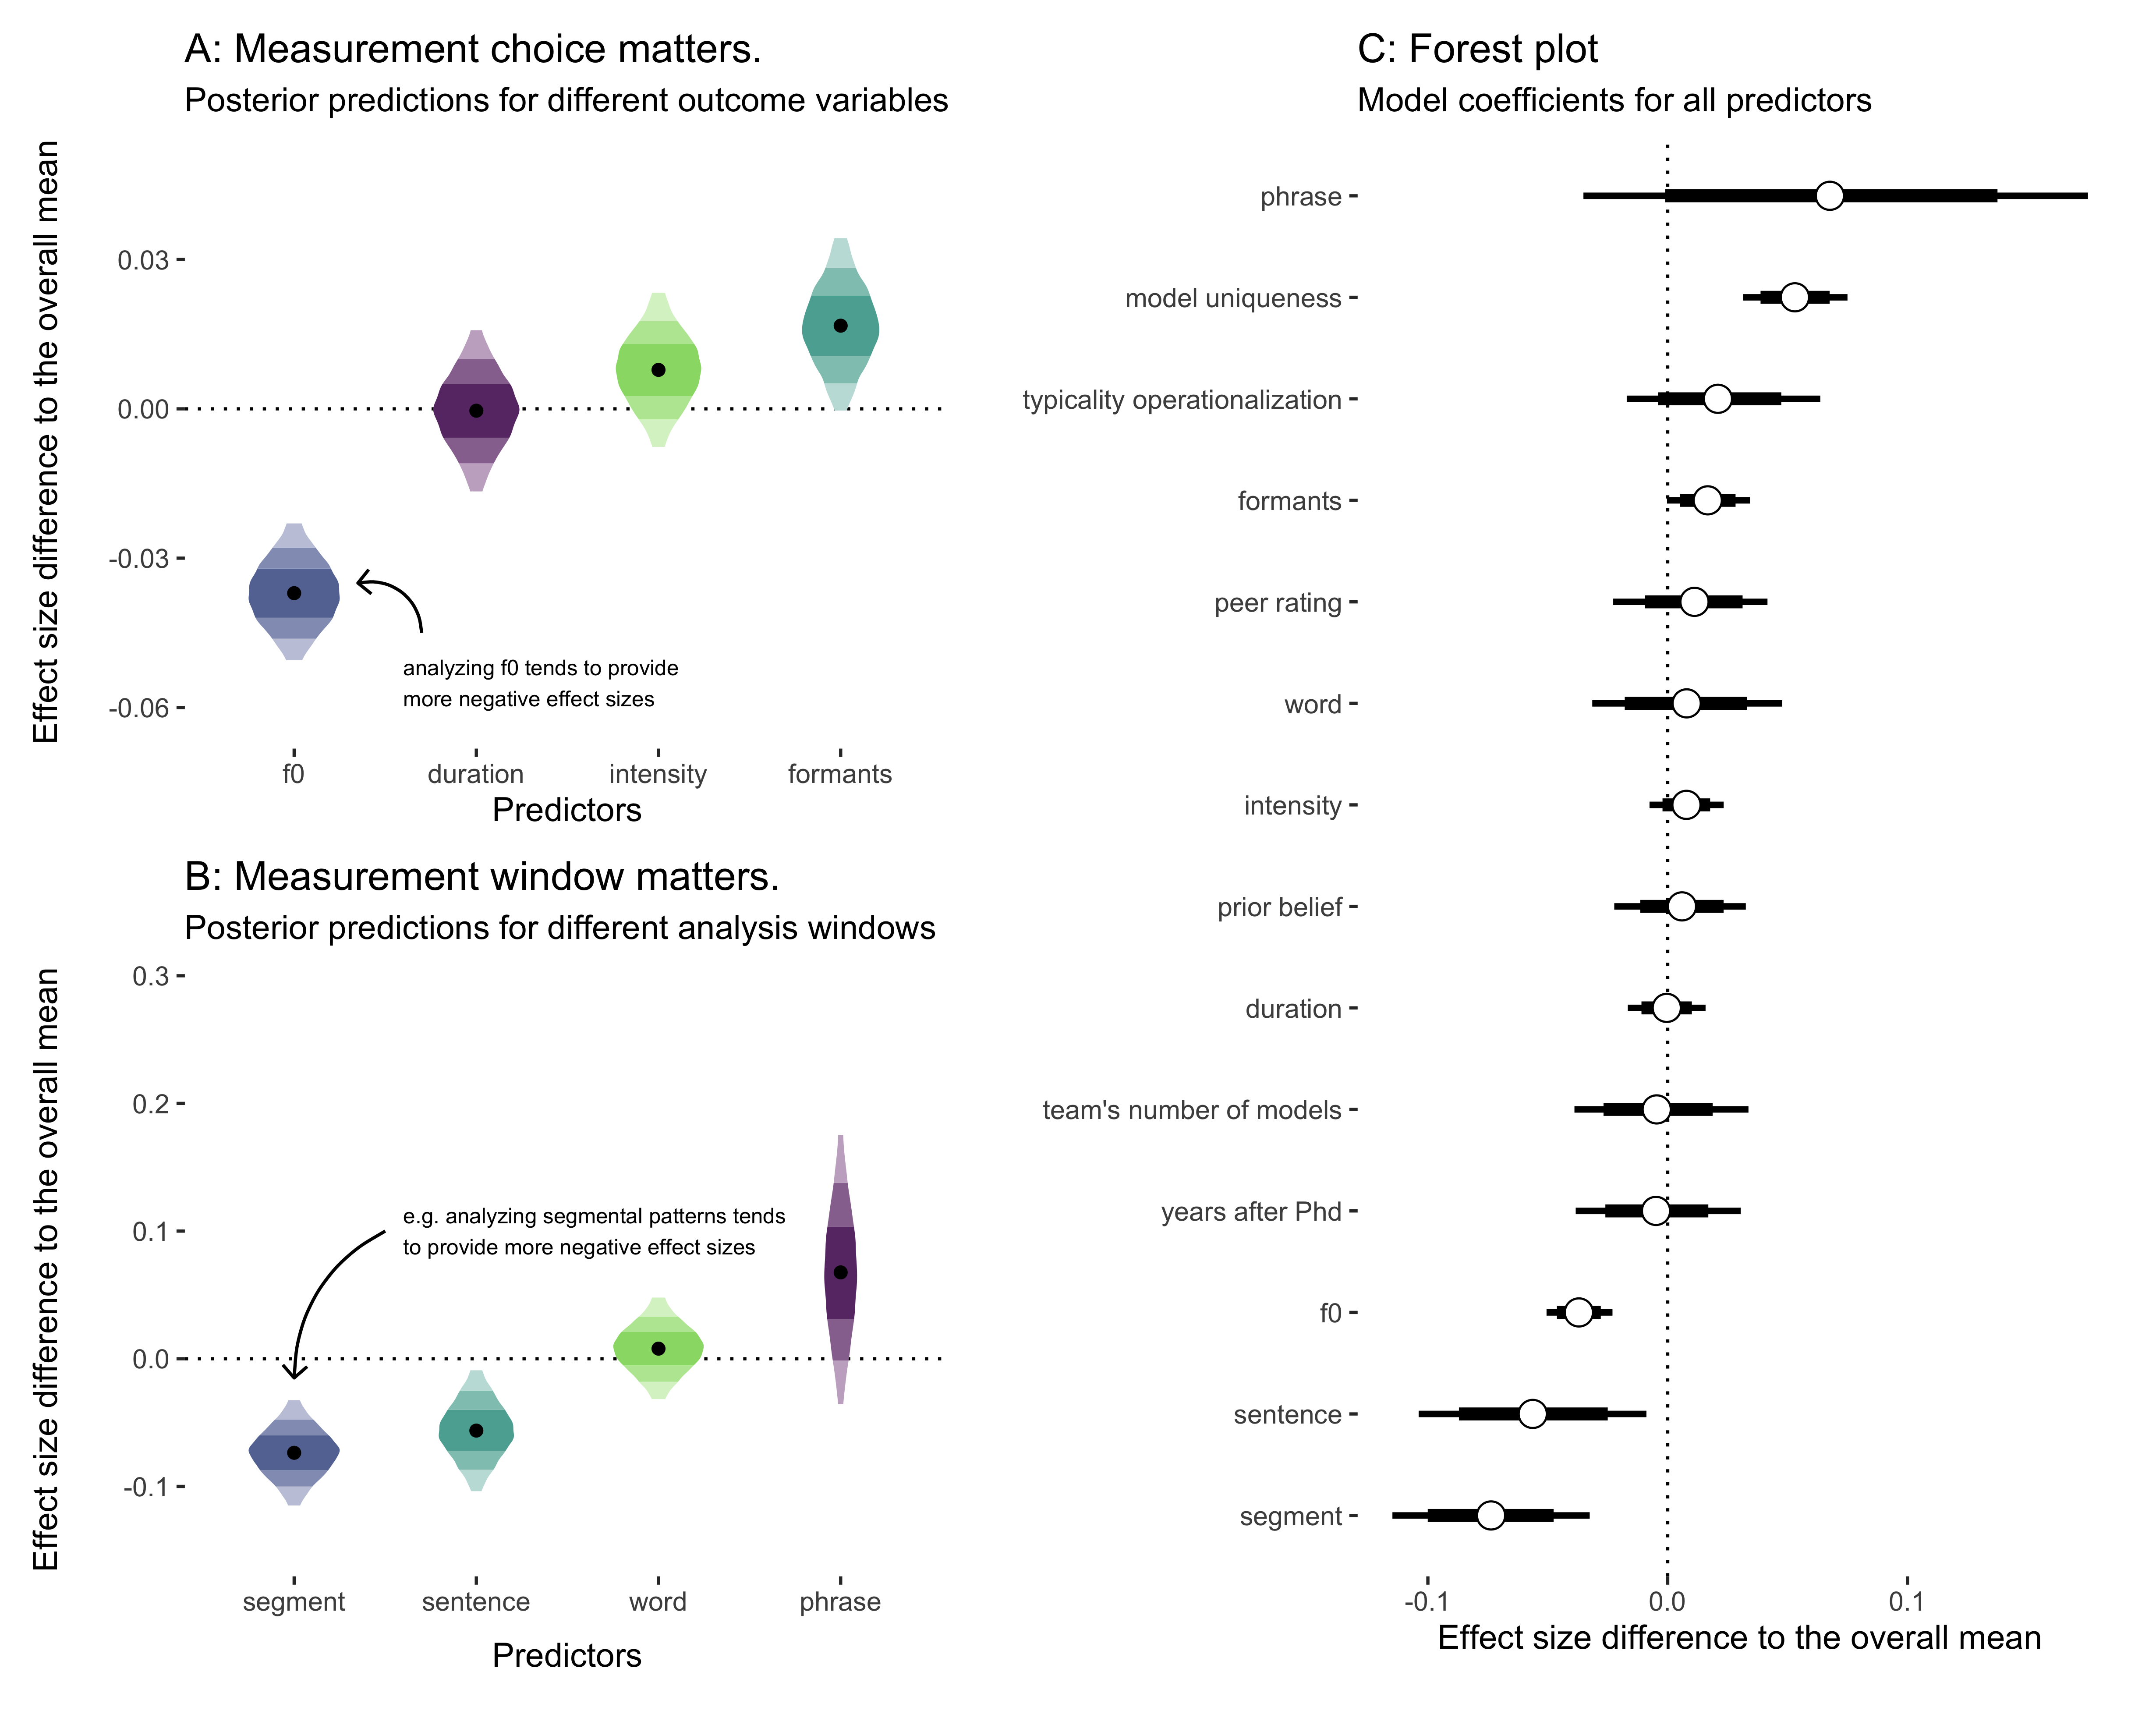
\includegraphics[width=1\linewidth]{../figs/alltogether} \caption{(ref:metaPlot2)}\label{fig:plot-meta2}
\end{figure}

\hypertarget{discussion}{%
\section{Discussion}\label{discussion}}

\hypertarget{summary}{%
\subsection{Summary}\label{summary}}

We gave XX analyst teams the same speech dataset to answer the same research question: \emph{Do speakers acoustically modify utterances to signal atypical word combinations?}.
In order to answer this question, teams had to operationalize latent variables within a multidimensional signal, operationalize and chose appropriate predictors, and construct an appropriate statistical model to answer the research question.
As shown by the results of this meta-analytic study, such complex process has led to a wide ``garden of forking paths'', i.e.~to a wide range of combinations of possible analytical decisions.
Every individual analyst team has chosen unique paths to acoustically measure, operationalize and statistical analyse the data.
Interestingly, the observed variation in reported effect sizes was not predicted by the analysts' prior expectations about the phenomenon.
In fact, teams on average rated the plausibility of the effect as rather high before receiving access to the data.
The variation in reported effect sizes was neither predicted by the analysts' experience in the field nor by the perceived quality of the analysis as judged by other teams.
Analyses received overall high peer ratings for both the acoustic and the statistical analysis, suggesting that reviewers were generally satisfied with the other teams' approaches.
These findings are very much in line with previous crowd-sourced projects that suggest variation between teams is neither driven by perceived quality of the analysis nor by analysts biases or experience \citep[e.g.,][\citet{breznau2021observing}]{silberzahn2018many}.
Given the mounting evidence, \citet{breznau2021observing} conclude that ``{[}\ldots{]} we are left to believe that idiosyncratic uncertainty is a fundamental feature of the scientific process that is not easily explained by typically observed researcher characteristics or analytic decisions.''
Idiosyncratic variation across researchers might be a fact of life which researchers have to acknowledge and integrate into how they evaluate and present evidence.

While properties of the teams did not seem to systematically affect results, teams' estimates seem to depend on certain measurement choices.
Human speech is a complex multidimensional signal.
Researchers need to make choices about what to measure, how to measure it and which temporal unit to measure it in.
Some outcome choices seem to bias the estimates in our data in one direction while others seem to bias estimates into another.
For example, measurements related to fundamental frequency tended to result in lower estimates while measurements related to vowel formants tended to yield higher estimates.
This asymmetry can have several causes.
First, there could be a true underlying relationship between typicality and the speech signal that manifests itself in some measures but not others and/or manifests itself negatively in one acoustic measure but positively in another.
Second, certain measurement choices might be associated with stronger expectations relative to the research question, which might lead to strong biases.
Many researchers targeted measures related to voice fundamental frequency (f0) since similar functional relationships like information structure and predictability can be expressed via f0 \citep[e.g.][]{grice2017integrating, turnbull2017role}.
Third, ADD REASONS.
Regardless of its cause, we have to conclude that depending on the choice of how the speech signal is operationalized, researchers might find evidence for or against a theoretically relevant effect.

It particularly struck us that teams did not follow our instructions to only submit a single effect size.
Teams submitted up to 16 different models to test for a possible relationship between typicality and the speech signal.
Obviously, the complexity of the speech signal lends itself to multiple approaches, but this plurality of hypothesis tests invites bias and can dramatically increase the rate of falsely claiming the presence of an effect \citep{roettger2019researcher}.
When operating within the frequentist inferential framework, testing the same hypothesis with different dependent variables, increases the Type-I error rate if not corrected for \citep[Tukey 1953,][]{benjamini1995controlling}.
It also invites bias, possibly leading to the selective reporting of those tests that yield a desirable outcome \citep[\citet{john2012measuring}, \citet{simmons2011false}]{kerr1998harking} while null results remain unreported \citep[e.g.,][\citet{rosenthal1979file}]{sterling1959publication}.

\hypertarget{lessons-for-the-methodological-reform-movement}{%
\subsection{Lessons for the methodological reform movement}\label{lessons-for-the-methodological-reform-movement}}

The current results point to important barriers for successful accumulation of knowledge.
The replication crisis has brought attention to scientific practices that lead to unreliable and biased claims in the literature {[}e.g., REFERENCE{]}.
One of the suggested paths forward is for researchers to directly replicate previous study more often \citep[e.g.,][]{open2015estimating, camerer2018evaluating}.
While we agree with the importance of direct replications, our study (and similar crowd-sourced analyses before us) suggest that replicating more is simply not enough.
There is only limited value in learning that a particular procedure is replicable if the idiosyncratic nature of the procedure itself might not yield a representative result relative to all possible procedures that could have been applied to the research question.
The quantitative sciences are in an inference crisis \citep{rotello2015more, starns2019assessing}.
Well-trained and experienced speech researchers not only applied completely different approaches to the same research question, they also seemed to consider all these alternative approaches acceptable, as their peer-ratings suggest.
Being aware of this idiosyncratic variation between analysts should lead to more nuanced claims and what Breznau et al.~refers to as ``epistemic humility''.

A desired outcome of knowing that different but reasonable measurement choices or statistical approaches might lead to entirely different interpretations of research data is to calibrate our (un)certainty in the strength of the collected evidence and, in turn, communicate that (un)certainty appropriately.
The fact that the choice of measurement, measurement window, and predictor choice affect the answer to the research question further suggests that research assumptions and hypotheses should be formulated with much greater detail, particularly so in regards to how measurement systems (here, the acoustic signal) and underlying conceptual constructs (here, the phonetic expression of typicality) relate to each other.
We should ideally specify the link between conceptual construct and quantitative system---the ``derivation chain'' \citep{dubin1970theory, meehl1990summaries}---prior to data collection and analysis, including defining constructs and their relationship within the quantitative system, specifying auxiliary assumptions and boundary conditions, and defining target measurements, statistical expectations and possible (and impossible) effect magnitudes.
Without well defined derivation chains, we ``are not even wrong'' \citep{scheel2022most} because falsified expectations cannot tell us much about the conceptual constructs they are based on when the relationship between the two is underspecified.

In light of the observed analytic flexibility, what can we do to appropriately calibrate our confidence in our claims?
First of all, through sharing of materials, data and statistical protocols, we can make our idiosyncratic choices transparent to others \citep{munafo2017manifesto, vazire2017quality}.
It further enables the evaluation and verification of underlying claims and allows for the evaluation of empirical, computational and statistical reproducibility (LeBel et al., 2018).
It allows for alternative analyses to establish analytic robustness (Steegen et al., 2016) and strengthens attempts to synthesize evidence via meta-analyses (Nicenboim et al., 2018)
This enables critical evaluation and robustness checks by other fellow researchers (REF).
Given that minor procedural changes can sometimes drastically affect the final interpretation of the results \citep{breznau2021observing}, we should ideally share a detailed documentation of the data collection procedure, the measurement choices, the data extraction, and statistical analyses.
Within fields that deal with speech data, open source software that allows to extract acoustic parameters via reproducible scripts can help other researchers to trace back seemingly inconsequential choices during the measurement process {[}e.g., CITE Praat, EMU CITE){]}{]}.

ADD

Second, making analytic pathways completely re-traceable does not change the fact that analysts apply different analytic approaches.
Crowd-source projects such as the current one can shed light on the range of degrees of freedom during analysis and help producing a consensual estimated effect using meta-analytic techniques.
This is obviously not always feasible in terms of required resources and time, but could be a consideration for claims that have large epistemological or practical consequences.

Third, if researchers have a good understanding of relevant analytic degrees of freedom, they could apply all conceivable analytic strategies and compare the results across all combinations of these choices.
This approach is called ``multiverse analysis'' \citep[e.g,][]{steegen2016increasing, harder2020multiverse} and has recently gained popularity across disciplines.
Finally, neither crowd-sourcing nor multiverse analyses will guarantee that all relevant pathways are explored.
Crowd-sourcing is limited by the sampled analysts and their biases.
Multiverse analysis is limited even further by the one group of researchers who define possible analytic pathways.
Eventually, a mature scientific discipline should develop a set of detailed quantitative hypotheses of how conceptual constructs manifest themselves in the measured system, i.e.~in the present case how communicative pressures of functions are expressed in the acoustic signal.
This can be achieved by formalizing verbal expectations mathematically or using computational models \citep[e.g.,][]{van2020formalizing, guest2021computational, scheel2021hypothesis, devezer2021case}.

\hypertarget{caveats}{%
\subsection{Caveats}\label{caveats}}

Our study has several limitations that need to be considered when evaluating our results.
First, there is potential for bias. The coordinating authors have engaged with metascientific research before and have been actively involved in methodological debates about scientific practices including transparency and statistical methods. We have in the past used the lack of standardized analytical approaches as an argument for proposing behavior and policy changes in the field.
This might have biased our own judgment during the analysis which itself came with many researcher degrees of freedom.
We hope we were able to make these degrees of freedom as well as the timing and reasoning of our analytical choices detectable.
However, our results should be independently re-analysed and replicated using a different research question.
Moreover, our sample is an opportunity sample.
We have advertised the project through online platforms which might have led to the exclusion of certain potential researcher groups.
Moreover, while the number of participating teams is larger than most earlier crowdsourcing projects, it is likely to be too small to estimate meta-analytic estimates reliably.
This is particularly important for the predictor evaluation.
Since predictor levels were not systematically distributed across teams, our estimates are characterized by large uncertainty.
This uncertainty is possibly further inflated by the fact that he research question presented to the teams was vague: \emph{Do speakers acoustically modify utterances to signal atypical word combinations?}
Interpreting the research question/hypothesis differently in terms of its statistical consequences has recently been shown to explain some variation between analysis teams in many-analysis projects \citep{auspurg2021has}.
However, we consider this very underspecification of research hypotheses in the field of speech science (and beyond, see \citet{scheel2022most}) a common phenomenon.
For example, researchers seem to have not yet agreed on how to acoustically measure cross linguistically common phenomena such as word stress \citep[e.g.][]{gordon2017acoustic}.
- We have not investigated researcher positionality, which is known to be an important factor.

Despite these possible sources of uncertainty and bias, our study suggest that at a minimum we can expect the between-team variability that we have observed, which is quite substantial and possibly amplifying biases.

Second, the generalizability of our findings to other disciplines on the one hand and specifically other sub-disciplines of the language sciences is, of course, limited.
Our focus was on quantitative analyses that require operationalization of a multidimensional signal. While some of our results can be informative for other disciplines working with speech or video signals, they are not very informative for expected variation between analysts working in qualitative fields of research.
This is an important point to make because the cognitive sciences in general, and the language sciences in particular have many research areas that are explored with qualitative methods. It is conceivable that the issues raised here to apply differently or not at all to qualitative data analysis.

\hypertarget{conclusion}{%
\section{Conclusion}\label{conclusion}}

\hypertarget{author-contributions}{%
\section{Author contributions}\label{author-contributions}}

See image at LINK {[}for peer-review, see figure \texttt{credit-taxonomy.png} attached with submission{]}.

\hypertarget{conflicts-of-interest}{%
\section{Conflicts of interest}\label{conflicts-of-interest}}

We have no conflicts of interest to disclose.

\appendix

\hypertarget{glossary}{%
\section{Glossary}\label{glossary}}

\begin{itemize}
\tightlist
\item
  \textbf{Analysis team}: team of analysts or single analyst.
\item
  \textbf{Reported effect sizes}: effect sizes reported by each analysis team.
\item
  \textbf{Standardized model}: Bayesian refit of the team's model.
\item
  \textbf{Standardized effect sizes}: (\(\eta_i\)) effect sizes returned by the standardized models.
\item
  \textbf{Standardized standard error}: (\(\text{se}_i\)) standard deviation of the standardized effect sizes.
\item
  \textbf{Bayesian random-effects meta-analysis} and \textbf{meta-analytic model}: multilevel intercept-only regression model for meta-analysis.
\item
  \textbf{Meta-analytic group-level standard deviation}: (\(\sigma_{\alpha_{\text{t}}}\)) standard deviation of the group-level effect of team returned by the meta-analytic model.
\item
  \textbf{Analytic and researcher-related predictors}: predictors used in the model that assess the effect of analytic and researcher-related factors on the standardized effects.
\end{itemize}

\bibliographystyle{sageh}
\bibliography{references}


\end{document}
